\documentclass[conference]{IEEEtran}
\IEEEoverridecommandlockouts
% The preceding line is only needed to identify funding in the first footnote. If that is unneeded, please comment it out.

% --- PACKAGES FOR TABLES, FIGURES, AND MATH ---
\usepackage{cite}
\usepackage{amsmath,amssymb,amsfonts}
\usepackage{algorithmic}
\usepackage{graphicx}
\usepackage{textcomp}
\usepackage{xcolor}
\usepackage{booktabs} % For professional-looking tables
\usepackage{hyperref} % For clickable links (optional)
\usepackage{siunitx}  % For aligning numbers by decimal point and handling units/signs
\usepackage{placeins}
\usepackage{tikz}
\usepackage{longtable}
\usepackage{adjustbox}
\usetikzlibrary{shapes.geometric, arrows}

\def\BibTeX{{\rm B\kern-.05em{\sc i\kern-.025em b}\kern-.08em
    T\kern-.1667em\lower.7ex\hbox{E}\kern-.125emX}}

\begin{document}

% --- TITLE AND AUTHOR INFORMATION ---
\title{Beyond Pruning and Dropout: Evolving Robust Networks via Persistent Stochastic Ablation
% \thanks{This work was supported in part by...} % Uncomment and fill if you have funding
}

\author{\IEEEauthorblockN{Tim Cotten}
\IEEEauthorblockA{\textit{Scrypted Inc.}, \textit{George Mason University}\\
tcotten@scrypted.ai, tcotten2@gmu.edu}
}

\maketitle

% --- ABSTRACT AND KEYWORDS ---
\begin{abstract}

This paper introduces and empirically evaluates ``Persistent Stochastic Ablation (PSA),'' a novel training paradigm that simulates evolutionary pressure via a ratcheting meta-learning process. At each cycle, PSA corrupts a pristine copy of the network's best-performing state (its ``Last Known Good'' state) through random neuron ablation. This damaged model is then trained against the last best performance benchmark on the validation dataset. A successful outcome promotes the newly trained model to become the next LKG state, effectively ``ratcheting'' the performance baseline upwards. This ``frustration'' mechanism forces repeated recovery attempts from a disadvantaged state, driving the model to escape difficult local optima or find more robust regularization solutions. Using a custom meta-learning harness, we conduct an systematic study on feed-forward Multi-Layer Perceptron (MLP) architectures ``SimpleMLP'' across a landscape of varying width, depth, and parameter counts on the MNIST dataset. Our findings reveal that the efficacy of PSA is not universal but is highly contextual. We trained 98 model configurations with six modes in a 3 vs. 3 comparison of baseline regularization techniques versus PSA: \{'None' (Control), 'Weight Decay', 'Dropout'\} and \{'Full', 'Hidden', 'Output'\}. For each combination we performed 10 randomly seeded trainings for a total of 5,880 total trial results. We identified and characterized four distinct behavioral training regimes: Beneficial Regularization, Optimally Sized, Chaotic Optimization, and Architectural Failure. These regimes are dictated by the interplay between model capacity and architectural stability; we document the regimes where PSA methods are beneficial, harmful, or indistinguishable compared to the existing control or regularization techniques, such as in over-parameterized models where 'Dropout' dominates. Further, we find a non-regularization use of PSA as a stochastic ``kick'' for low-capacity or exotic models to escape local minima that weight decay and dropout cannot rescue. By analyzing the temporal dynamics of model improvement, we demonstrate that can PSA act as a sustained, exploratory search mechanism, capable of achieving late-stage breakthroughs in otherwise intractable optimization landscapes. Crucially, this initial study is limited by the fundamental restrictions of the \texttt{SimpleMLP} architecture due to the boundaries of the Vanishing Gradient Problem, beyond which deeper topologies become untrainable, thereby establishing the necessary groundwork for future research with more robust architectures like a ResMLP with skip connections.
\end{abstract}

\begin{IEEEkeywords}
Neural Network Regularization, Ablation Studies, Evolutionary Algorithms, Deep Learning, Vanishing Gradient Problem, Local Minima, Model Capacity, Model Stability, Multi-Layer Perceptron (MLP), Stochastic Optimization, Meta-Learning, Network Robustness, Fault Tolerance
\end{IEEEkeywords}


% --- SECTIONS OF THE PAPER ---

\section{Introduction}

Deep neural networks, despite their demonstrable power, remain susceptible to two fundamental issues: becoming trapped in poor local minima during optimization, and a tendency to learn brittle feature representations due to overfitting in over-parameterized architectures. Conventional ablation methodologies to combat these challenges fall into two dominant paradigms: \textbf{post-hoc pruning} \cite{b1, b2} for computational efficiency, and \textbf{transient regularization}, like Dropout \cite{b3}, to prevent feature co-adaptation during training.

This study investigates a third paradigm of ablative techniques in deep learning we term \textbf{Persistent Stochastic Ablation (PSA)}. Unlike its predecessors, PSA is not motivated by efficient reduction of network size or preventing immediate co-adaptation of features. Nor does it rely on post-hoc analysis and pruning. Instead, it leverages \textit{blind, iterative harm} as a continuous, online training driver. 

We hypothesize that by repeatedly forcing a network to recover from non-strategic damage to its best-performing state, we can simulate a virtual evolutionary pressure, and that this pressure can manifest in at least two ways: first, by acting as a powerful stochastic search mechanism, capable of ``kicking'' ill-conditioned models out of poor local minima, and second, by encouraging more robust and fault-tolerant feature representations. This concept is inspired by Neural Darwinism\cite{b4}, wherein stochastic variation and selection drive adaptive neural development.

To test this hypothesis, we developed the ``Frustration Engine,'' a meta-learning framework that implements the PSA training loop. The process is a simple, powerful ratchet: 1) A pristine copy of the network's best state (the ``Last Known Good'' or LKG) is corrupted via random neuron ablation. 2) This damaged model is trained against the LKG's performance benchmark. 3) If successful, the new state becomes the next LKG.

\begin{figure}[h!]
\centering
\resizebox{\columnwidth}{!}{%
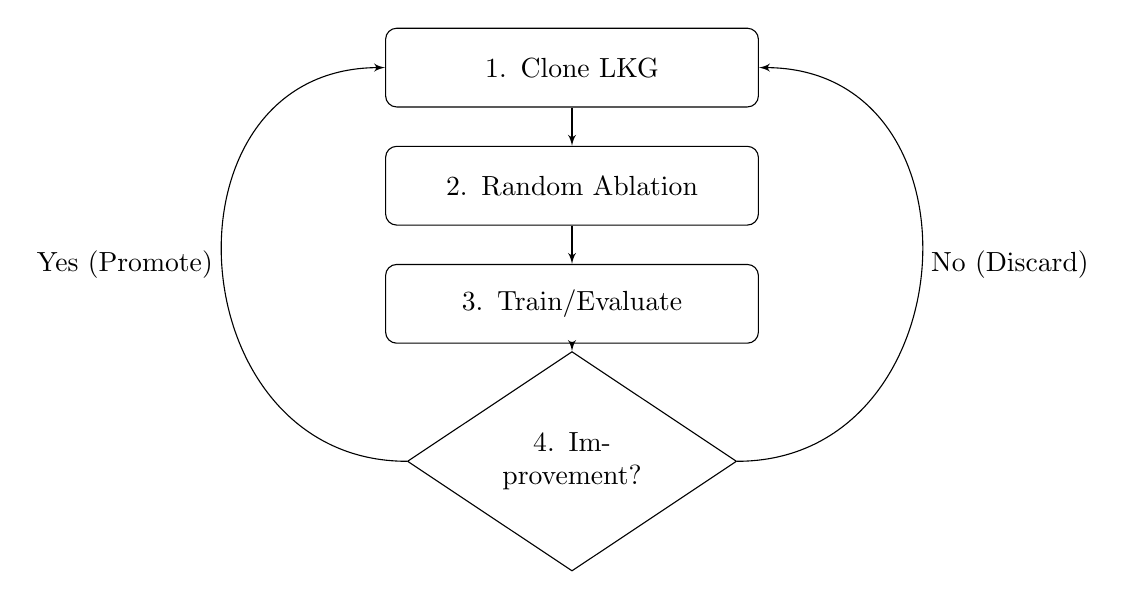
\begin{tikzpicture}[
    node distance=1.5cm,
    auto,
    >=latex',
    block/.style={draw, rounded corners, text width=4.5cm, text centered, minimum height=1cm},
    decision/.style={draw, diamond, aspect=1.5, text width=2.5cm, text centered}
]
    % Node placement
    \node (lkg) [block] {1. Clone LKG};
    \node (ablate) [block, below of=lkg] {2. Random Ablation};
    \node (train) [block, below of=ablate] {3. Train/Evaluate};
    \node (promote) [decision, below of=train, node distance=2cm] {4. Improvement?};
    
    % Arrows
    \path[->] (lkg) edge (ablate);
    \path[->] (ablate) edge (train);
    \path[->] (train) edge (promote);
    
    % Feedback Loops
    \path[->] (promote) edge [out=0, in=0, looseness=1.5] node[right] {No (Discard)} (lkg);
    \path[->] (promote) edge [out=180, in=180, looseness=1.5] node[left] {Yes (Promote)} (lkg);

\end{tikzpicture}%
}
\caption{The conceptual flow of the Persistent Stochastic Ablation (PSA) meta-loop. On failure, the process discards the candidate and starts a new cycle from the unchanged LKG state. On success, the challenger is promoted to become the new LKG.}
\label{fig:psa-flow-vertical}
\end{figure}

This ``meta-loop'' design continuously forces the model to recover from a disadvantaged state, fundamentally differing from Dropout, which applies transient noise that is discarded after each weight update within a single training epoch. In contrast, the ``damage'' and ``recovery'' from PSA is persistent between successful training cycles, forcing a structural, rather than merely statistical, adaptation.

Utilizing an outer loop that guides an inner learning process is a cornerstone of meta-learning, established by works like Model-Agnostic Meta-Learning (MAML) \cite{b6} for few-shot adaptation. Our proposed strategy is thus inspired by MAML-like meta-learning paradigms, not for cross-task adaptation, but for guiding the optimization of a single model on a single task despite the ``frustration'' of iterative corruption, using a ratcheting mechanism to capture learning opportunities.

This initial study documents our exhaustive experiments on a simple Multi-Layer Perceptron (MLP) architecture using ReLU activation neurons, mapping its response to PSA across a wide range of architectures defined by varying capacity and stability. This study seeks to answer three fundamental questions:

1. Under what conditions, particularly in cases of architectural instability or optimization failure (e.g. the Vanishing Gradient Problem\cite{b5}), can PSA provide a unique benefit by enabling escape from otherwise intractable local minima?

2. In what regimes does PSA act as a competitive regularizer, and when does it become an irredeemably detrimental source of damage compared to established techniques like Weight Decay or Dropout, or even the control?

3. Can we demonstrably disentangle the effects of online neural ablation via PSA depending on the affected layers, specifically differentiating and measuring the effects of stochastically operating on hidden layers, the output layer, or all of them combined?

\section{Methodology}

Our methodology is designed to rigorously evaluate Persistent Stochastic Ablation (PSA) across a wide experimental landscape. All trials were conducted within our ``Frustration Engine'' meta-learning framework to ensure controlled and fair comparisons between training paradigms. The experiment is structured along two orthogonal axes. The first axis compares three PSA modes (\verb|Full|, \verb|Hidden|, and \verb|Output|) against a baseline group of three standard training methods: a no-intervention control (\verb|None|), \verb|Weight Decay|, and \verb|Dropout|. The second, architectural axis tests these six modes across a curated landscape of 98 distinct Multi-Layer Perceptron (MLP) topologies on the MNIST dataset. Each of the resulting 588 combinations was trained 10 times with independent random seeds, yielding 5,880 total trials. This large-scale design provides the statistical power necessary to move beyond anecdotal results, allowing us to isolate the influence of model capacity and architectural stability, and to characterize the distinct behavioral regimes that emerge from the interplay between each strategy and the network it attempted to train.

\subsection{Experimental Landscape}

To disentangle the effects of network topology from raw parametric capacity, we designed our experimental landscape around the principle of \textbf{parameter matching} and \textbf{mirrored configurations}. Using our experimental \verb|SimpleMLP| testbed, we curated a collection of 98 homogeneous architectures (L*W) that systematically explore the 2D space of network depth (L) and width (W), as visualized in Figure \ref{fig:simplemlp_design_space}.

First, we created a distribution of architectural configurations of \verb|1*W| networks, where 2 $\le$ \verb|W| $\le$ 2048. We then extended this to deeper ``shallow-and-wide'' configurations (e.g., \verb|2*W|, \verb|4*W|) by solving for a width \textbf{\textit{W}} that approximately matched the parameter count of a \verb|1*W| counterpart (ex.\{\verb|1*2048|, \verb|2*939|, \verb|4*632|\} having \{\verb|1,628,170|, \verb|1,629,175|, \verb|1,702,618|\} parameters).

To do this, we first used the standard formula for determining the parameters of an MLP:
\begin{equation}
P_{total} = H_1(N_{in}+1) + \sum_{i=1}^{L-1}H_{i+1}(H_i+1) + N_{out}(H_L+1)
\label{eq:params}
\end{equation}
where $N_{in}=784$ and $N_{out}=10$. Then, we solved for a width approximation formula based on the target parameter count \textbf{\textit{P}} and fixed number of layers \textbf{\textit{L}}:\\

\begin{equation}
\adjustbox{width=\columnwidth,center}{$W_{\text{target}} \approx
\frac{-(794 + L_{\text{target}}) + \sqrt{(794 + L_{\text{target}})^2 + 4(L_{\text{target}}-1)(P_{\text{base}} - 10)}}{2(L_{\text{target}}-1)}$}
\label{eq:param_matching_final}
\end{equation}
\\\\
Second, we created ``square'' network architectures of shape \verb|L*W| where \verb|L=W| in order to explore deeper topologies, still solving for parameter matching using the previous formula (ex. \verb|115*115| being 1,612,195 parameters to match \verb|1*2048|).

\begin{figure}[ht]
    \centering
    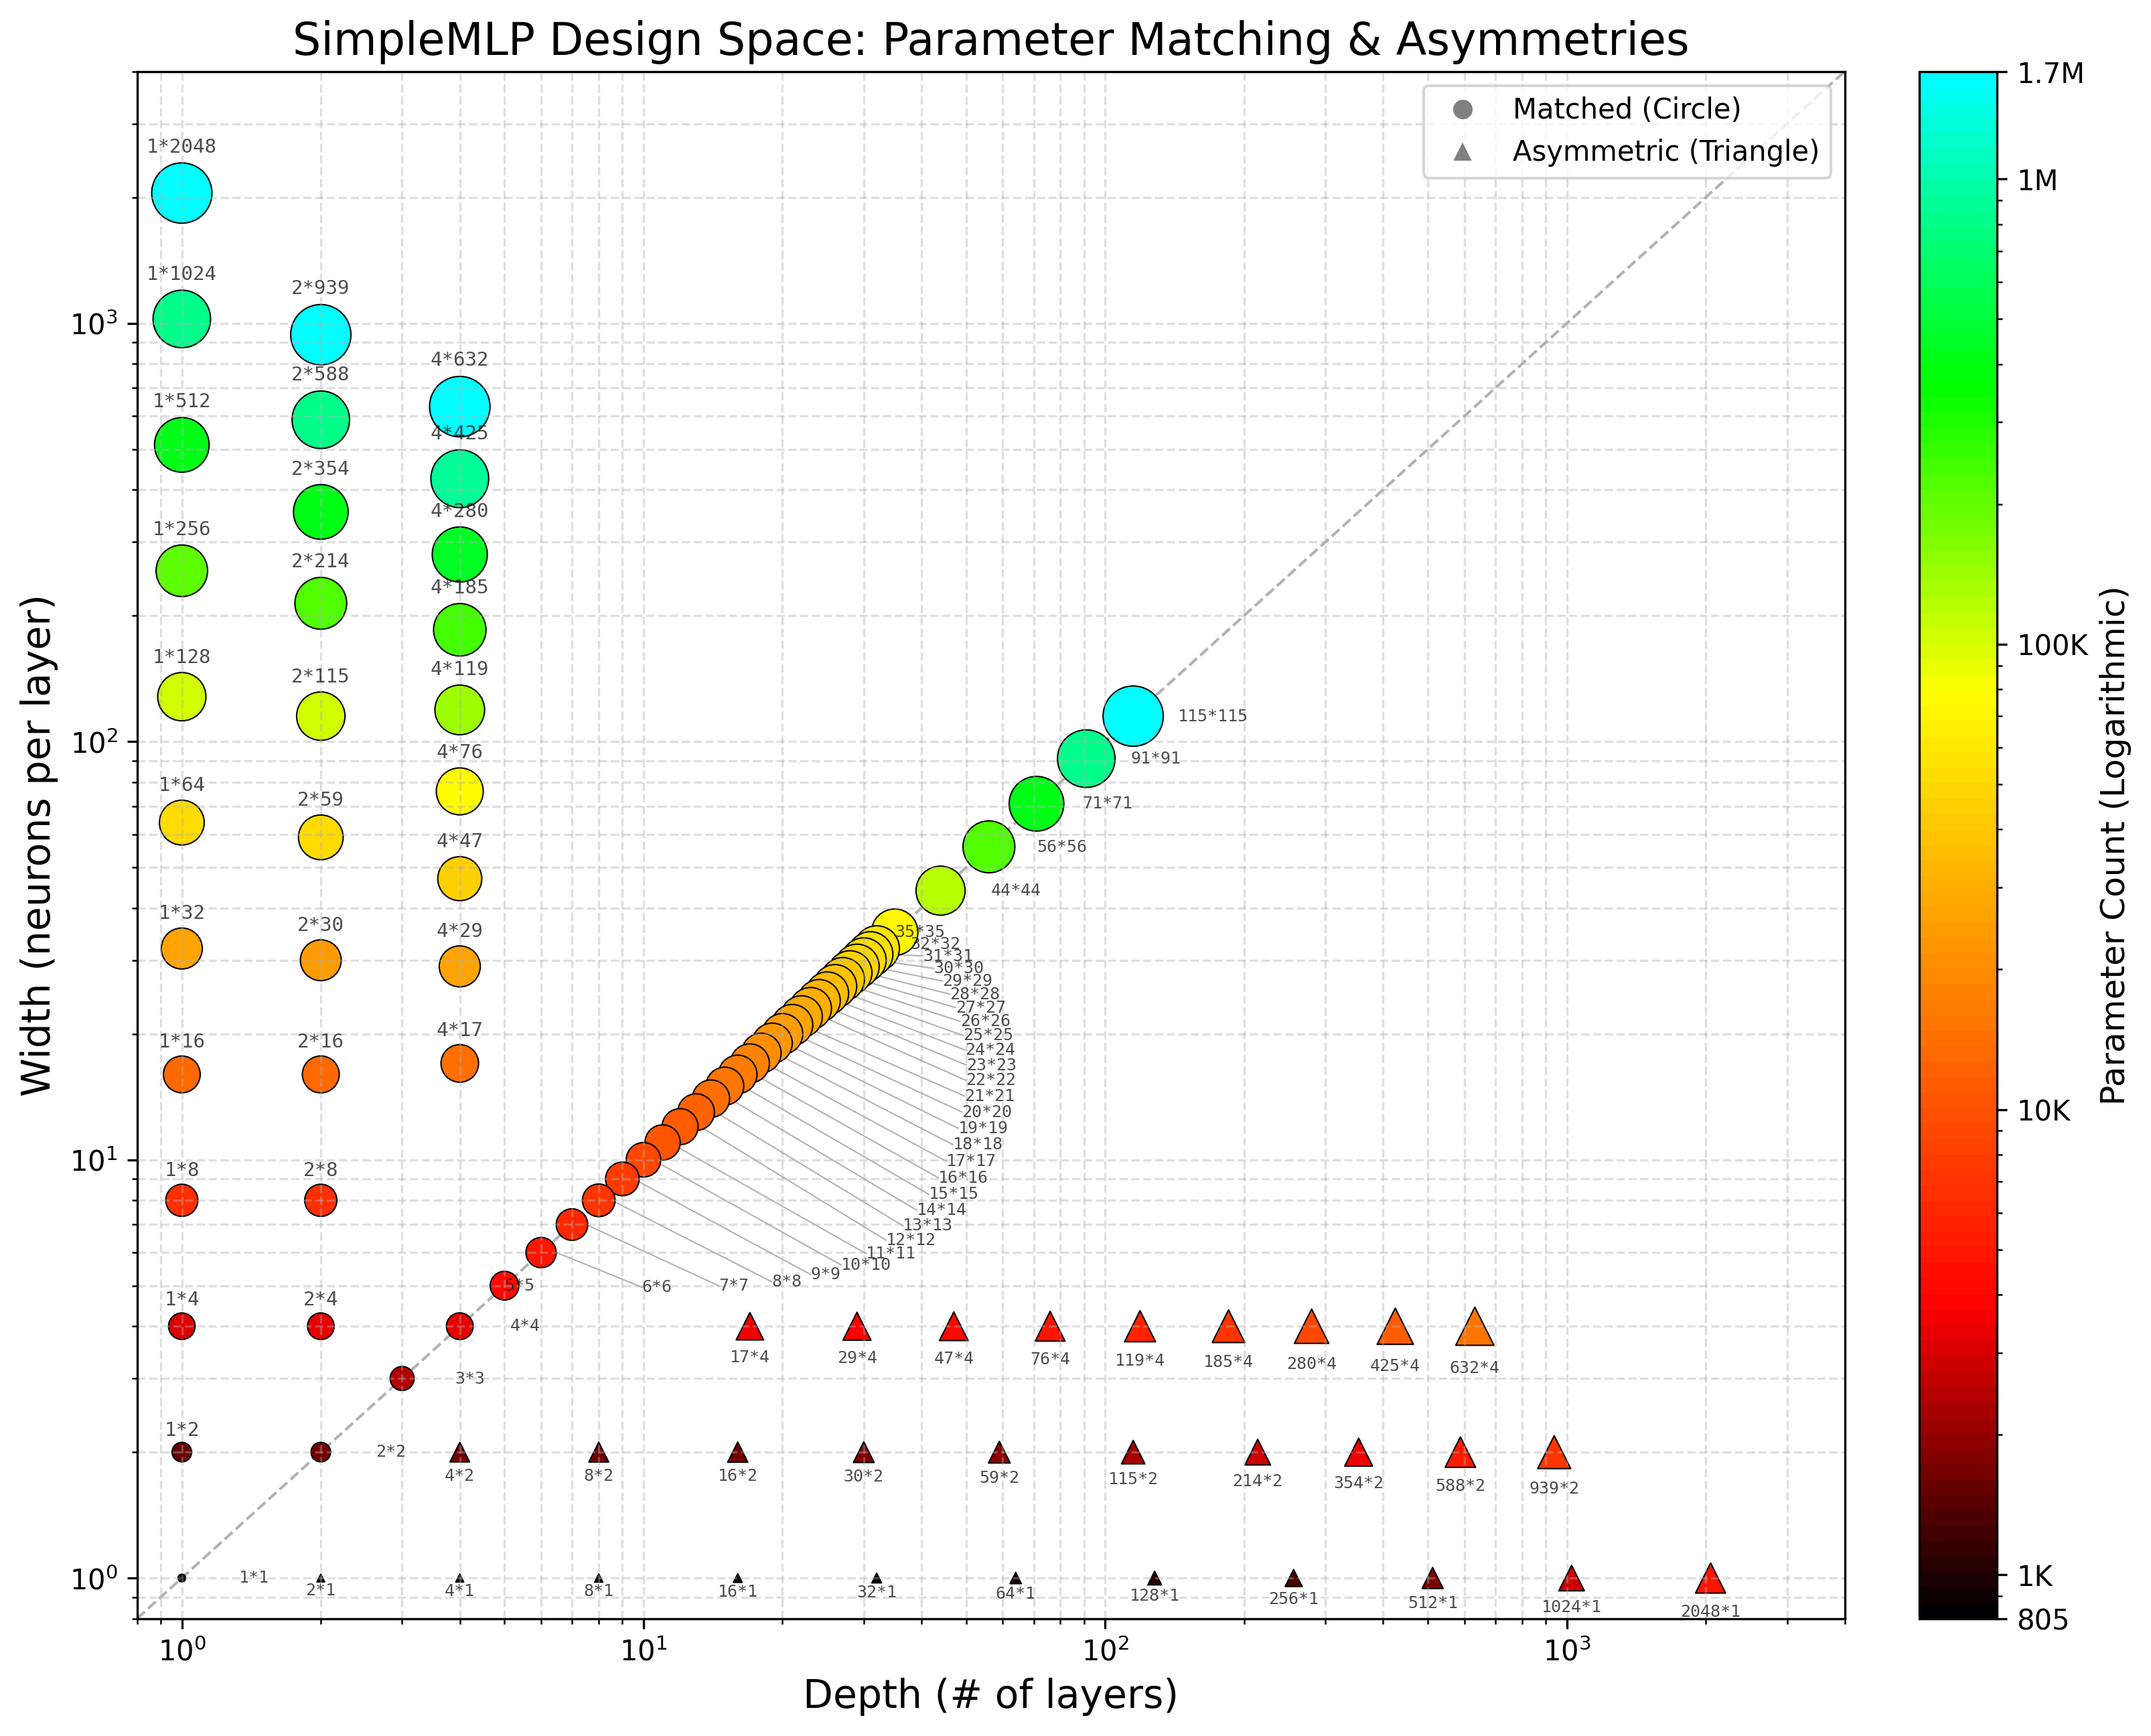
\includegraphics[width=\linewidth]{SimpleMLP_Heatmap_Parameter_Matching.png}
    \caption{The architectural design space, illustrating our principles of parameter matching and asymmetry. Architectures in the shallow-and-wide (top-left) and square (diagonal) regions are parameter-matched (circles), with size indicating total parameters. Asymmetric deep-and-narrow configurations (triangles) are included to explore the boundaries of trainability.}
    \label{fig:heatmap_param_matching}
\end{figure}

Third, we mirrored the ``shallow-and-wide'' network configurations into their inverted ``deep-and-narrow'' opposites, such as adding \verb|16*4| to complement \verb|4*16|. We deemed these \textbf{asymmetric}, as we couldn't feasibly design parameter matching equivalents along the mirrored axis, opting instead to invert the \verb|L*W| relationship to \verb|W*L| (ex. we added \verb|256*1| to complement \verb|1*256|). We did this with the full understanding that such pathological networks were not viably trainable, but felt it was valuable to experiment on them nonetheless.

Finally, in order to identify the behaviors of the baselines and ablative techniques as deeper networks failed due to the Vanishing Gradient Problem (VGP), we created additional parametrically asymmetric square designs to fill the entire space between \verb|1*1| and \verb|32*32|.

% SimpleMLP design space figure
\begin{figure*}[ht]
\centering
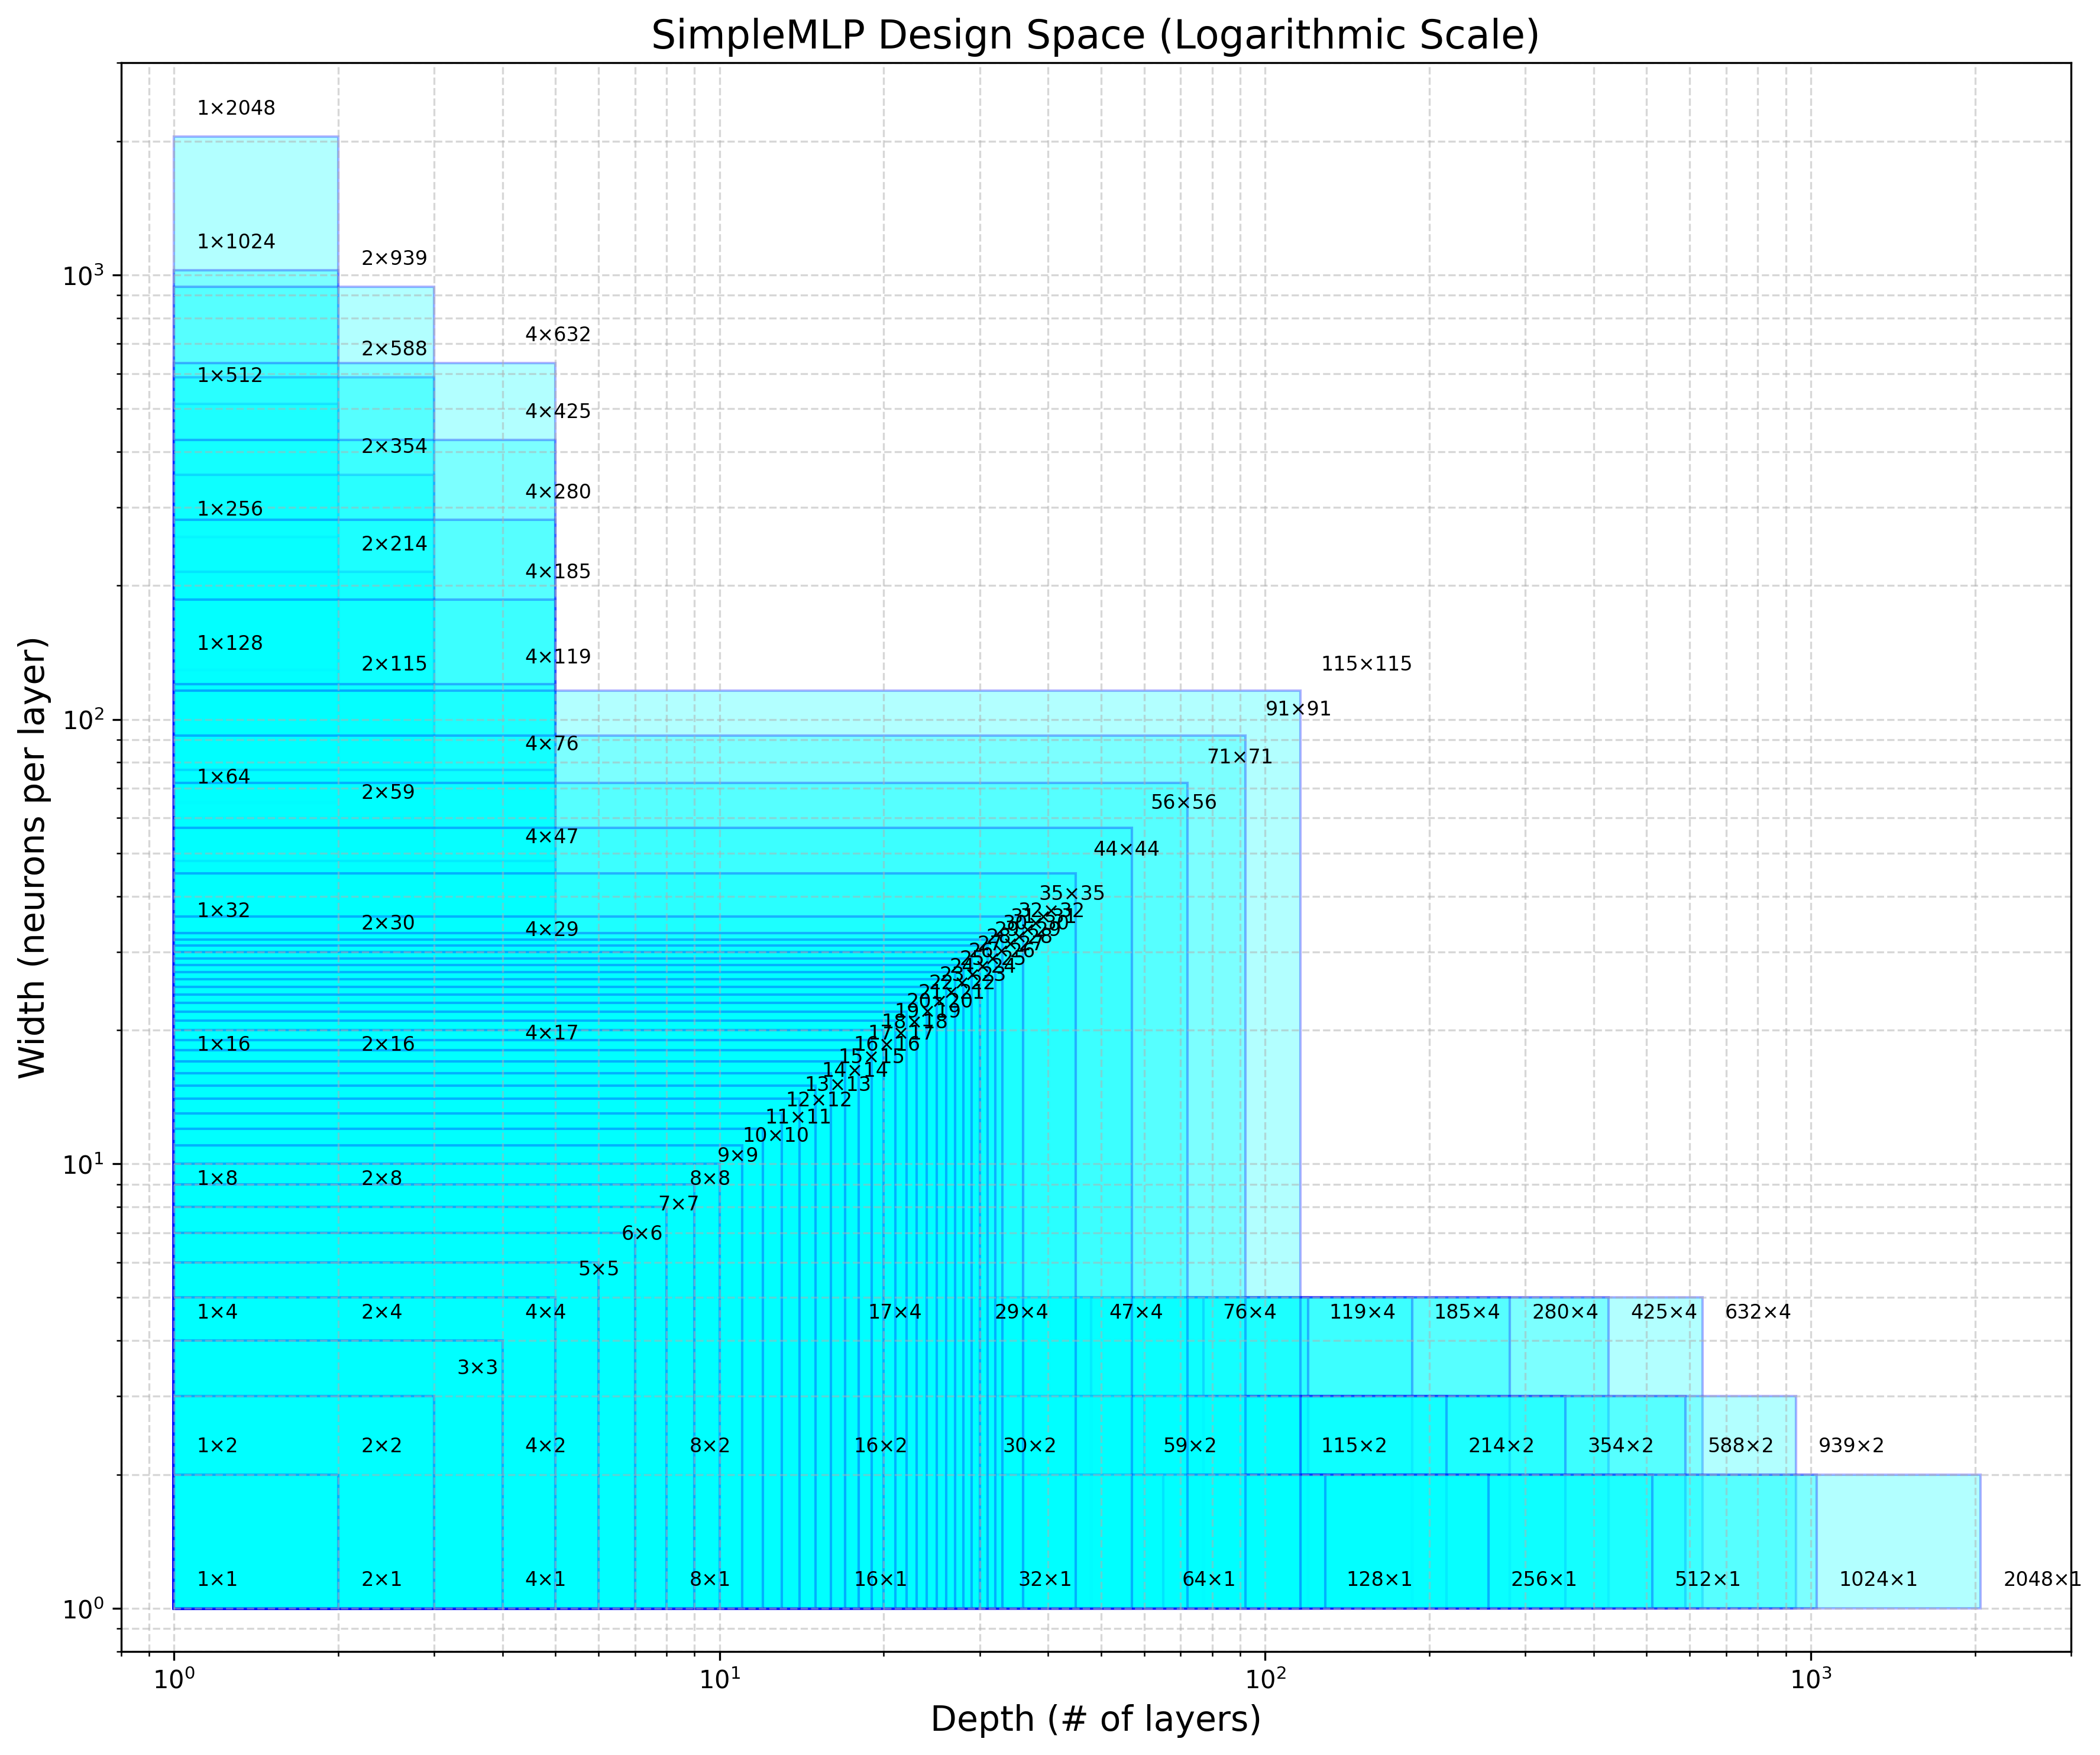
\includegraphics[width=\columnwidth]{SimpleMLP_Testing_Design_Space.png}
\caption{The SimpleMLP architectural design space, visualized on a logarithmic scale. Width (neurons per layer) is plotted on the Y-axis, and depth (number of layers) is plotted on the X-axis. This visualization clearly demonstrates the exploration range from shallow-and-wide architectures (\texttt{1*2048}) to square architectures (\texttt{115×115}) and degenerate deep-and-narrow configurations (\texttt{2048*1}).}
\label{fig:simplemlp_design_space}
\end{figure*}

The full test suite is documented in the Appendix: Table~\ref{tab:architecture_parameters}

\subsection{The SimpleMLP Testbed}

The experimental testbed for this study is a feed-forward Multi-Layer Perceptron (MLP), termed \verb|SimpleMLP|, designed to be dynamically configured from a single command-line argument (\verb|--arch|).

\verb|SimpleMLP| is constructed as a sequence of hidden blocks, where each block consists of a \textbf{Linear} layer, followed by a \textbf{Rectified Linear Unit (ReLU)} activation, and a \textbf{Dropout} layer. Blocks are defined in the form \verb|L*W| where \verb|L| represents the number of layers and \verb|W| the width of each layer in neuron count. The network's final layer is a linear output head that maps the final hidden state to 10 output logits for MNIST classification. The forward pass for an input \textit{\textbf{x}} and \textit{\textbf{L}} hidden layers is defined as: 

\begin{align}
h^{(0)} &= \text{Flatten}(x) \\
h^{(i)} &= \text{Dropout}(\text{ReLU}(W_i h^{(i-1)} + b_i)) \quad \text{for } i=1, \dots, L \\
y_{\text{logits}} &= W_{\text{out}} h^{(L)} + b_{\text{out}}
\end{align}
where $h^{(i)}$ is the output of the $i$-th hidden block, and $W$ and $b$ represent the weight matrices and bias vectors for their respective layers.

To ensure a fair comparison, \verb|nn.Dropout| modules are included in the model graph for all configurations. These layers are only active during training when \verb|--ablation-mode| is explicitly set to \verb|dropout|; in all other modes, they are set to evaluation mode and function as identity operators. We do not include them when calculating parameters, and this design guarantees that the number of trainable parameters remain identical across all experimental conditions: isolating the behavioral effects of the chosen regularization or ablation strategy within any given architectural design.

Thus, a given MNIST training architecture can be summarized as:

\begin{align*}
\text{Input (784-dimensional)}\\
&\rightarrow [\text{Linear} \rightarrow \text{ReLU} \rightarrow \text{Dropout}] \times N \\
&\rightarrow \text{Linear (10 neurons)} \rightarrow \text{Output}
\end{align*}

\subsection{Flexible Architectural Design}

The \verb|SimpleMLP| architecture also allows multiple collections of hidden blocks to be stacked in sequence to create complex arrangements, such as funnels (ex. \verb|[1*512, 2*256, 4*128, 8*64]|). To facilitate reproducible and large-scale experimentation, the architecture is defined via a compact string notation. For example, \verb|--arch "[2*128, 4*64]"| specifies a network with two hidden blocks of 128 neurons, followed by four hidden blocks of 64 neurons.

However, for the purposes of our study's experimental design we limited ourselves to homogeneous network architectures such as \verb|(1*2048)|, \verb|(2*512)|, or \verb|(8*8)|. We reserve research on heterogeneous architectures like \verb|[2*128, 1x10, 4x16]| for our future work.

\subsection{The ``Frustration Engine''}
The core of our methodology is a meta-learning loop that iteratively challenges the network to improve upon its historical best performance. We define the ``Last Known Good'' (LKG) as the model state with the highest-ever validation accuracy, and the ``Bounty'' as that accuracy score. A single meta-loop consists of:
\begin{enumerate}
    \item \textbf{Clone LKG:} The cycle begins by cloning the weights of the current LKG model into a candidate model.
    \item \textbf{Ablation:} PSA is applied by permanently ablating a single, randomly-chosen neuron in the candidate model. Ablation consists of zeroing the incoming weights, the bias, and, if applicable, outgoing weights.
    \item \textbf{Train:} The newly damaged candidate model is trained for one full epoch.
    \item \textbf{Evaluate:} If the new model's accuracy exceeds the current Bounty, it becomes the new LKG, and its score is the new Bounty. Otherwise, the candidate model is discarded.
    \item \textbf{Repeat:} The process repeats from Step 1, ensuring improvements are only committed if the model successfully overcomes the damage.
\end{enumerate}

\begin{figure}[h!]
\centering
\begin{align*}
% Step 1: Create a damaged candidate from the LKG state
W_{\text{candidate}} &= \mathcal{A}(W_{\text{LKG}}^{(t)}) \\[1em]
% Step 2: Train the candidate to produce a new challenger state
W_{\text{challenger}} &= \mathcal{T}(W_{\text{candidate}}) \\[1em]
% Step 3: Evaluate the challenger's performance score
S_{\text{challenger}} &= \mathcal{E}(W_{\text{challenger}}) \\[1em]
% Step 4: Ratchet the LKG state for the next cycle (t+1)
W_{\text{LKG}}^{(t+1)} &=
\begin{cases}
W_{\text{challenger}} & \text{if } S_{\text{challenger}} > S_{\text{LKG}}^{(t)} \quad \text{(Promote)} \\
W_{\text{LKG}}^{(t)} & \text{otherwise} \quad \text{(Discard)}
\end{cases}
\end{align*}
\caption{The Persistent Stochastic Ablation (PSA) Meta-Learning Loop. The process iteratively corrupts the best-known state (\textit{LKG}) and challenges the network to recover and surpass its previous performance benchmark before a new state is promoted.}
\label{fig:psa-loop}
\end{figure}

Naturally, in the cases of the baseline training modes the ablative damage step is skipped, but otherwise the meta-loop proceeds in the same manner.

\subsection{Optimizer Resets}
To ensure a fair and direct comparison between the proposed PSA methods and established baselines (e.g., \verb|none|, \verb|weight decay| and \verb|dropout|), the optimizer state is reset at the beginning of each meta-loop. We felt allowing a persistent optimizer would be a confounding variable, as we only want to measure performance differences between the baseline/regularization and ablation strategies themselves, rather than benefit from any accumulated history within the optimizer's internal state (e.g., \textit{momentum}). We believe the concept of a persistent optimizer learning from failure while routing around ablative damage to be an avenue for future research.

\subsection{Deconstructing Training Effects}
To understand the mechanisms of PSA, we designed six distinct training modes in order to disentangle possible effects, half in a baseline group (\textbf{None}, \textbf{Weight Decay}, \textbf{Dropout}), the other half in a group specifically dedicated to PSA techniques (\textbf{Full}, \textbf{Hidden}, \textbf{Output}). 

\begin{itemize}
    \item \textbf{none (Control):} The baseline model with no intervention.\\
    \item \textbf{decay (Weight Decay):} Standard weight decay applied with a fixed constant rate.\\
    \item \textbf{dropout (Dropout): } Standard dropout applied with a fixed constant rate.\\
    \item \textbf{full (Blended Pressure):} Randomly chooses a hidden linear layer from within the hidden blocks or the output layer, then chooses a random neuron to ablate. All incoming weights and the neuron's bias are zeroed (\textbf{partial ablation}). This represents a combination of the effects of the \verb|hidden| and \verb|output| modes.\\
    \item \textbf{hidden (Internal Pressure):} Randomly chooses a neuron from the list of all neurons available in the hidden linear layers from with the hidden blocks, then performs a \textbf{full ablation} on it, where the incoming weights, bias, and \textit{outgoing} weights are zeroed.\\
    \item \textbf{output (External Pressure):} Randomly chooses a neuron from the linear output layer, then performs a \textit{partial} ablation on it.\\
\end{itemize}

\subsection{Data Pipeline and Scalable Training}

To ensure the rigor and reproducibility of our 5,880 trials, we implemented a data pipeline designed for consistency, performance, and methodological soundness. These design decisions guarantee that any observed performance differences are attributable solely to the architectural and training strategy variations under experimentation.

\subsubsection{Deterministic Dataset Splitting}

We deterministically partitioned the standard MNIST dataset, comprising 60,000 training and 10,000 testing images, using a static seed (\verb|1337|) to create a pseudo-random subset of 50,000 training images and 10,000 validation images from the original 60,000 image training set. The original 10,000-image test set was reserved for unbiased performance evaluation, and was unseen by the models being trained.

\subsubsection{In-Memory Data Loading}

Before training begins the entire MNIST dataset is loaded from disk once, converted into tensors, and stored in RAM. This eliminates the need for repetitive disk reads during the 100 meta-loops of each trial, greatly speeding up execution.

DataLoaders were configured with \texttt{num\_workers=0} to avoid unnecessary multiprocessing overhead and \texttt{pin\_memory=True} on CUDA-enabled systems.

\subsubsection{AWS SageMaker AI}

After validating the training process on multiple pieces of hardware, such as Apple Silicon (M3) and CUDA (NVIDIA A10G), we designed a set of project tools for utilizing Amazon Web Service's SageMaker AI to deploy hundreds of simultaneous training jobs.

We deployed 588 unique training jobs using \verb|ml.g4dn.xlarge| instances, each tasked with running 100 meta-loops, storing the logs, writing a summary file, deleting the intermediary model, and starting over from scratch for each trial, for a total of 10 trial runs per job. No explicit pseudo-random seeding was assigned to the trials, relying instead on default hardware randomization processes.

We then collected and aggregated all the CloudWatch logs as well as \verb|results.txt| summaries created by the SageMaker AI jobs, storing their data in the public repository as a reference for insights on the temporal dynamics of optimization during training and classification of validation results.

\subsection{Automated Regime Classification}

To ensure a reproducible analysis, we developed an automated, rule-based algorithm to classify each of the 98 architectures into one of four training regimes, based on the empirically observed performance and interactions of the six training modes. The algorithm applies a sequence of rules that operate on the summary statistics of the trial data.

The algorithm's failure threshold, $Z_{val}$, is not hard-coded but is dynamically determined by calculating the majority class baseline (ZeroR) accuracy of the MNIST validation set we set aside (empirically derived as $\sim11.02\%$).

Let $M$ be the set of all training modes, with subsets $B$ for baseline modes (\texttt{none}, \texttt{decay}, \texttt{dropout}) and $A$ for ablative modes (\texttt{full}, \texttt{hidden}, \texttt{output}). For each mode $m \in M$, let $\mu_m$, $\sigma_m$, and $P_m^{\text{(max)}}$ be its mean, standard deviation, and peak accuracy, respectively. The rules are applied in the following order:

\begin{enumerate}
    \item \textbf{Architectural Failure:} If all trials fail to exceed the validation ZeroR baseline then the model is untrainable.
    \begin{equation}
        \max_{m \in M} (P_m^{\text{(max)}}) \le Z_{val}
    \end{equation}

    \item \textbf{Beneficial Regularization:} The model is over-parameterized and all modes, including PSA, perform similarly: classified when the mean accuracy of all modes ($\mu_m$) is within one effective standard deviation, $\sigma_{eff}$, of the baseline mean ($\mu_B$). We define $\sigma_{eff} = \max(\sigma_B, 0.5\%)$ to establish a minimum tolerance for models with near-zero variance.
    \begin{equation}
        |\mu_m - \mu_B| \le \sigma_{eff} \quad \forall m \in M
    \end{equation}

    \item \textbf{Optimally Sized:} Regularization becomes detrimental as parametric capacity decreases, with PSA becoming actively harmful when compared to the baseline methods: classified when the mean accuracy of the ablative modes ($\mu_A$) is more than one effective standard deviation below the baseline mean.
    \begin{equation}
        \mu_A < (\mu_B - \sigma_{eff})
    \end{equation}

    \item \textbf{Chaotic Optimization:} If none of the above rules are met, the architecture is evaluated for whether it's ``chaotic'': characterized by either (a) the baseline modes failing ($P_b^{\text{(max)}} \le Z_{val}$ for all $b \in B$) while at least one ablative mode succeeds ($P_a^{\text{(max)}} > Z_{val}$ for some $a \in A$), or (b) the ablative modes providing a significant average performance uplift ($\mu_A > \mu_B + 0.5\%$).\\
    
\end{enumerate}

This algorithm successfully classifies all 98 architectures using the previous rules, and are visualized in (Figure~\ref{fig:regime_map}).

\section{Results: The Four Regimes of Training (on SimpleMLP)}
Our large-scale experiment, comprising 5,880 trials across 98 distinct MLP architectures, reveals that the efficacy of Persistent Stochastic Ablation is not universal but is instead governed by the interplay between a model's parametric capacity and its architectural stability, especially when compared to baseline techniques. We identified four distinct behavioral regimes, which are clearly demarcated in the architectural design space, as visualized in Figure \ref{fig:regime_map}.

\begin{figure*}[ht]
\centering
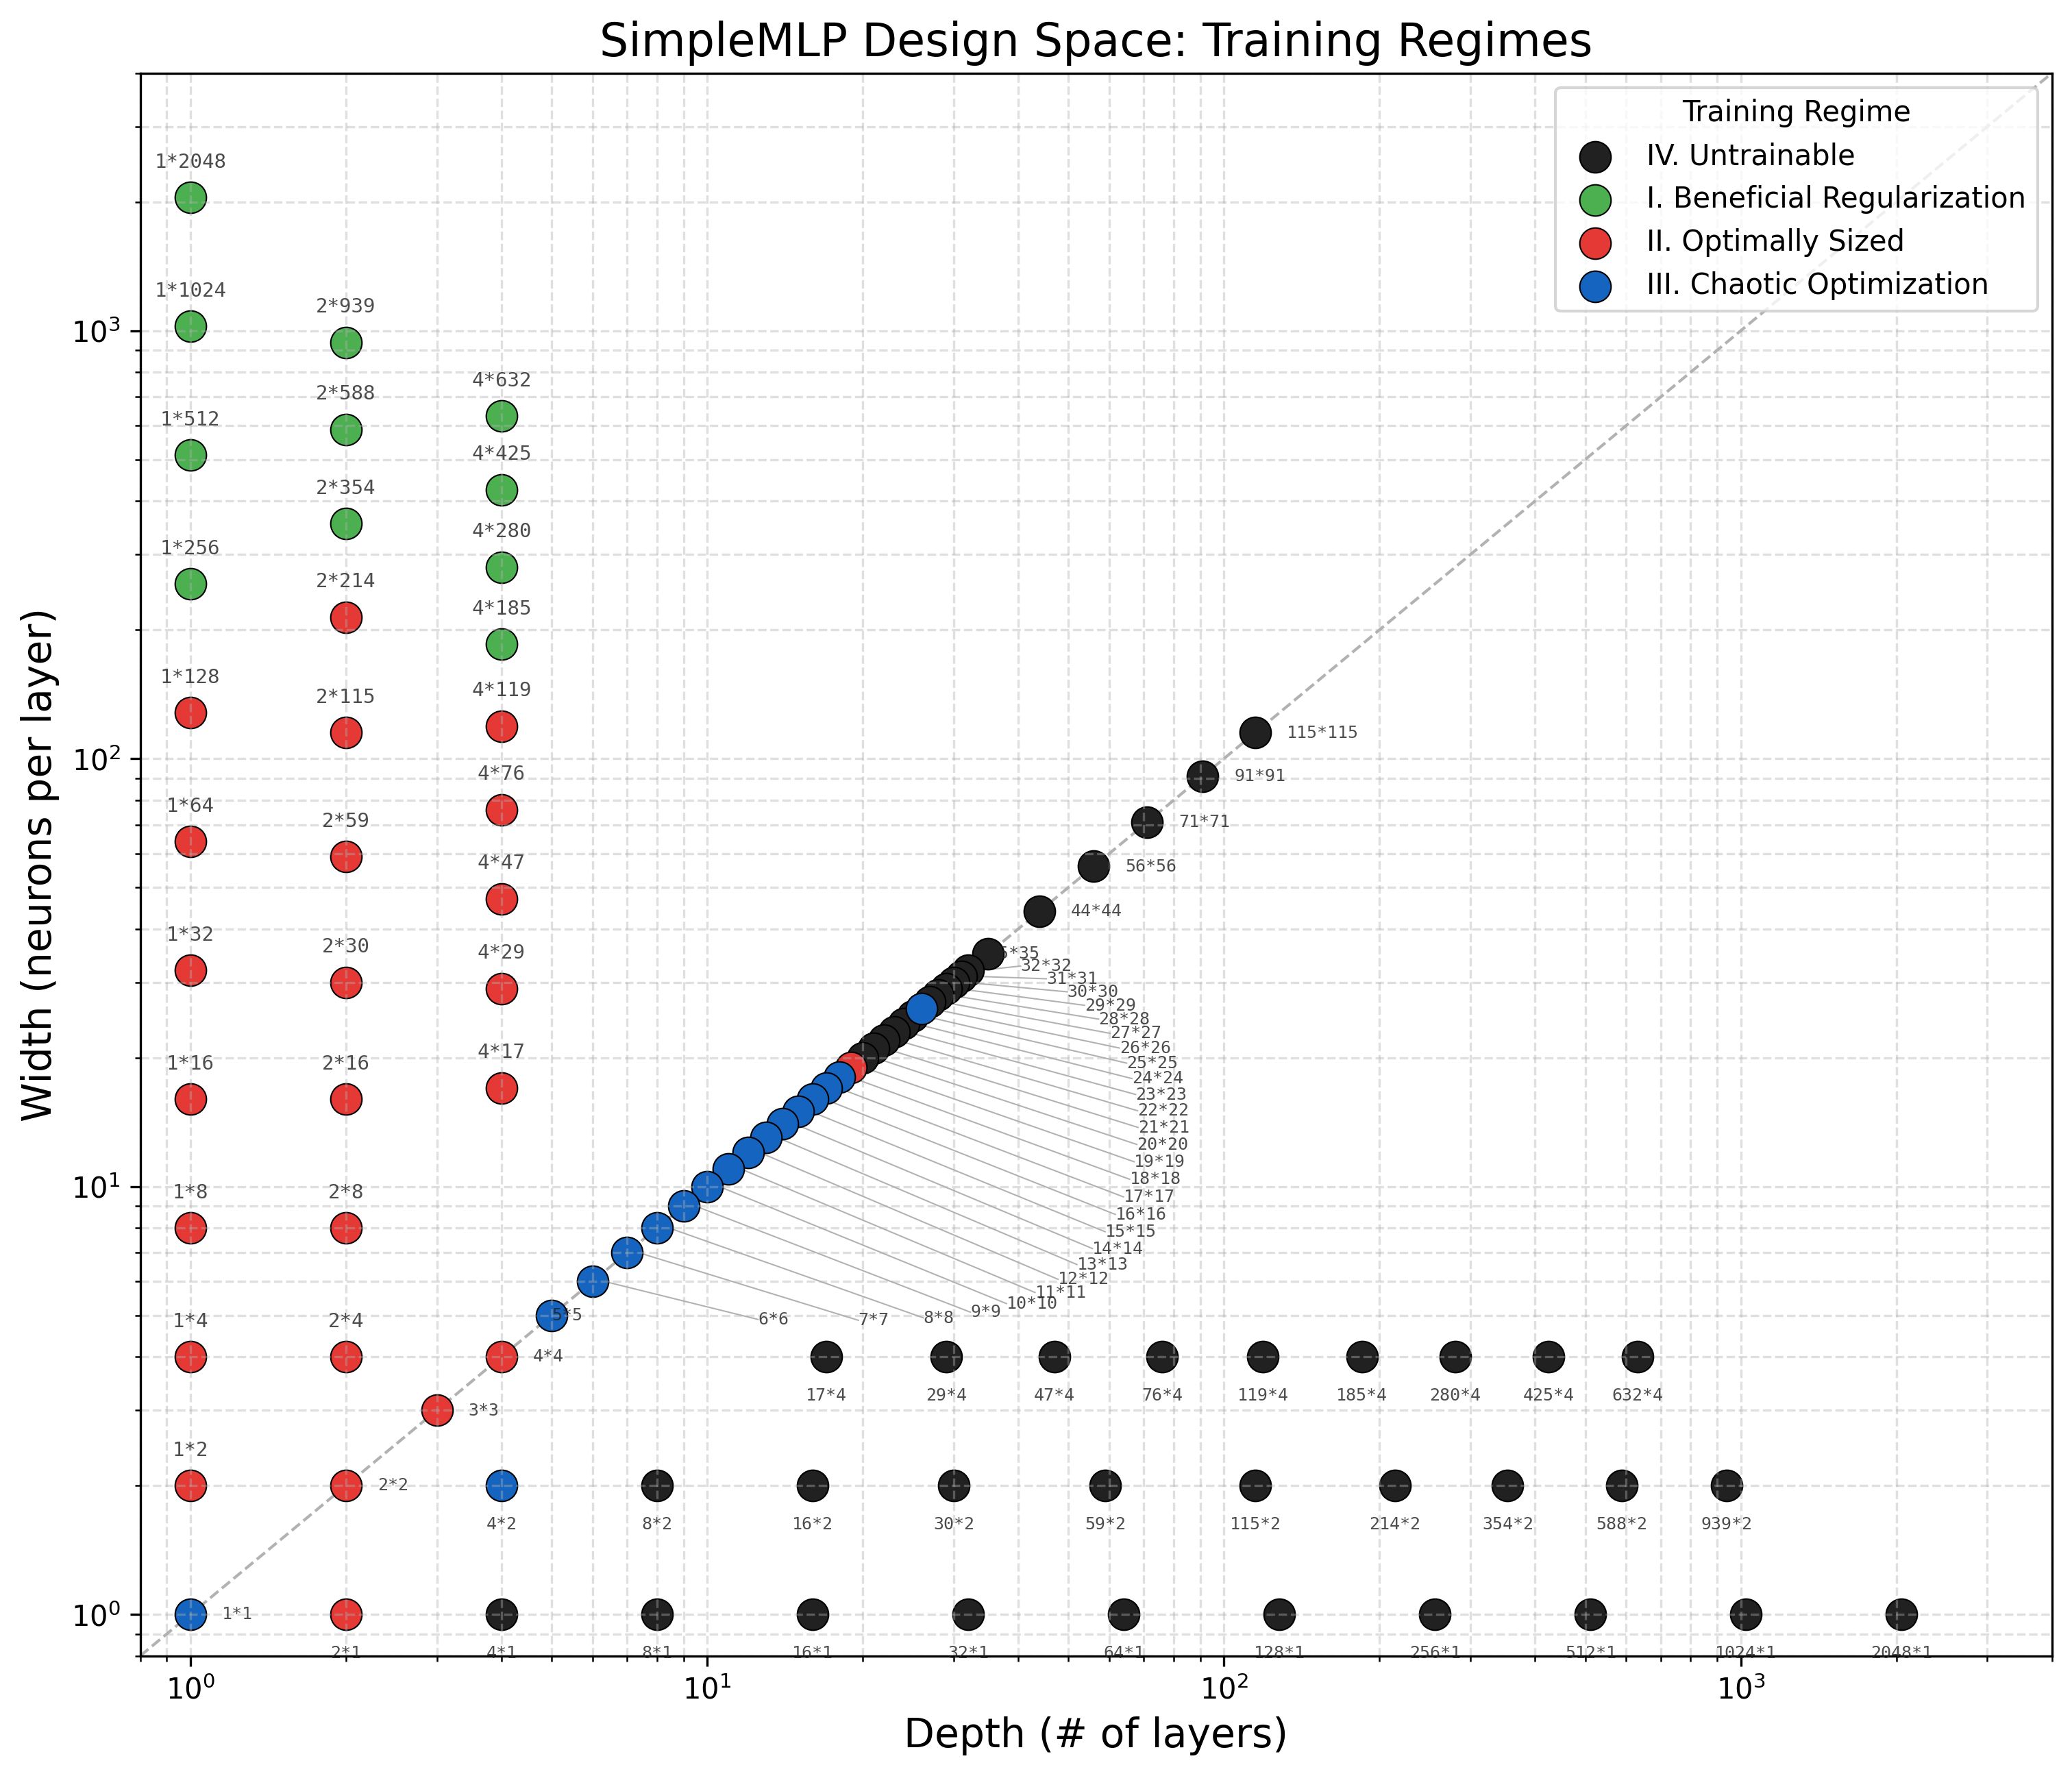
\includegraphics[width=\textwidth]{SimpleMLP_Heatmap_Regimes.png}
\caption{The four distinct training regimes identified across the SimpleMLP architectural design space. Each point represents an architecture, plotted by its depth and width on a log-log scale. The color indicates the emergent behavioral regime, revealing a clear relationship between model shape, capacity, and the effectiveness of different training strategies. The dashed diagonal line ($y=x$) separates shallow-and-wide from deep-and-narrow configurations, and also represents the boundary of intentional parameter matching.}
\label{fig:regime_map}
\end{figure*}

A summary of the training results for each model, over 10 trials each lasting for 100 meta-loops, is presented in the Appendix: Table~\ref{tab:results_summary}.

\subsection{Regime I: Beneficial Regularization in High Capacity, Stable Models}

Located in the upper-left quadrant of the design space (Fig. \ref{fig:regime_map}, green points), this regime consists of shallow-and-wide architectures with high parametric capacity (e.g., \texttt{1*2048}, \texttt{2*939}, \texttt{4*632}). These models are sufficiently over-parameterized for MNIST to easily overfit in a form of \textbf{Beneficial Regularization}.

In this regime, PSA also seems to function as a regularizer, but its blind damage is consistently outperformed by the more principled regularization of its baseline peers Dropout and Weight Decay. For the \texttt{1*2048} architecture with \texttt{1,628,170} parameters, for example, \textbf{Weight Decay} achieves the highest mean accuracy at \textbf{98.23\%}, demonstrating the most stable and reliable performance.

\begin{table}[h!]
\centering
\caption{Performance Summary for the \texttt{1*2048} Architecture\\ \texttt{1,628,170} Parameters (n=10).}
\label{tab:1x2048_results}
\begin{tabular}{lcccc}
\toprule
\textbf{Mode} & \textbf{Mean} & \textbf{Std} & \textbf{Min} & \textbf{Max} \\
\midrule
None    & 98.19\% & 0.06\% & 98.08\% & 98.34\% \\
Decay   & \textbf{98.23\%} & 0.03\% & 98.17\% & 98.26\% \\
Dropout & 98.19\% & 0.09\% & 98.06\% & 98.33\% \\
Full    & 98.13\% & 0.05\% & 98.04\% & 98.21\% \\
Hidden  & 98.22\% & 0.06\% & 98.15\% & \textbf{98.35\%} \\
Output  & 97.99\% & 0.09\% & 97.82\% & 98.11\% \\
\bottomrule
\end{tabular}
\end{table}

Interestingly, while traditional regularizers are superior on average, the stochastic nature of PSA allows it to occasionally discover outlier solutions. The \textbf{Hidden} ablation mode produced the single highest peak accuracy of this group at \textbf{98.35\%}, narrowly exceeding the maximums of all other methods. This suggests that while less reliable, PSA's random exploration can, by chance, find configurations inaccessible to more stable optimizers.

This trend becomes even clearer as depth increases. For the parameter-matched \texttt{2*939} architecture, \textbf{Dropout} emerges as the dominant strategy, securing both the highest mean accuracy (\textbf{98.23\%}) and the highest peak performance (\textbf{98.30\%}).

This demonstrates a clear hierarchy where principled regularizers are most effective, but the random search of PSA provides a different, albeit less consistent, performance profile.

A promising direction for future work is to analyze the convergence dynamics over time; our preliminary results suggest that \verb|dropout| converges most quickly (often in the first 50 meta-loops), followed by \verb|decay| and \verb|none|, while some PSA modes were still achieving performance improvements near the 100-meta-loop limit of our trials, hinting at a potentially longer but more exploratory optimization path.

\subsection{Regime II: Optimal Sizing in Low Capacity, Stable Models}

As model capacity decreases from the over-parameterized configurations, we enter a regime where the architectures are \textbf{Optimally Sized} for the MNIST task. These models (Fig. \ref{fig:regime_map}, red points), such as \texttt{1*128} or \texttt{2*59}, possess enough parameters to provide valuable solutions (e.g., with success rates $>$ 97\%) even without the significant parametric redundancy of their much larger counterparts.

The defining characteristic of this regime is that any training intervention, whether principled regularization or persistent ablation, becomes increasingly detrimental when compared to the control. Further, the maximum performance of PSA techniques diverge quickly from their baseline regularizing counterparts, with their damage becoming catastrophic far more quickly than their peers. 

In the \verb|1*256| configuration with \verb|203,530| parameters, sitting at the boundary between Beneficial Regularization and the Optimally Sizes regimes, the strongest PSA technique is \verb|hidden| with a maximum of 97.74\%, while the weakest baseline technique is \verb|decay| with a maximum of 97.90\% for a divergence of $\sim0.16\%$. Deeper into the regime, at the \verb|1*64| configuration with \verb|50,890| parameters, the maximums diverge significantly at $\sim0.84\%$ for \verb|hidden| and \verb|dropout|, at 96.23\% and 97.05\% respectively, illustrating the detrimental effects of PSA.

As shown in the ``Winning Strategy Map'' (Fig. \ref{fig:heatmap_winning}), there is a clear shift away from Dropout and Weight Decay being the top performers towards the None (Control) model as parameter counts drop towards less stable regimes. This indicates that the networks require their full parameter budget to function, and preserving every weight is the optimal strategy when the architecture is already optimally sized.

\begin{figure}[ht]
\centering
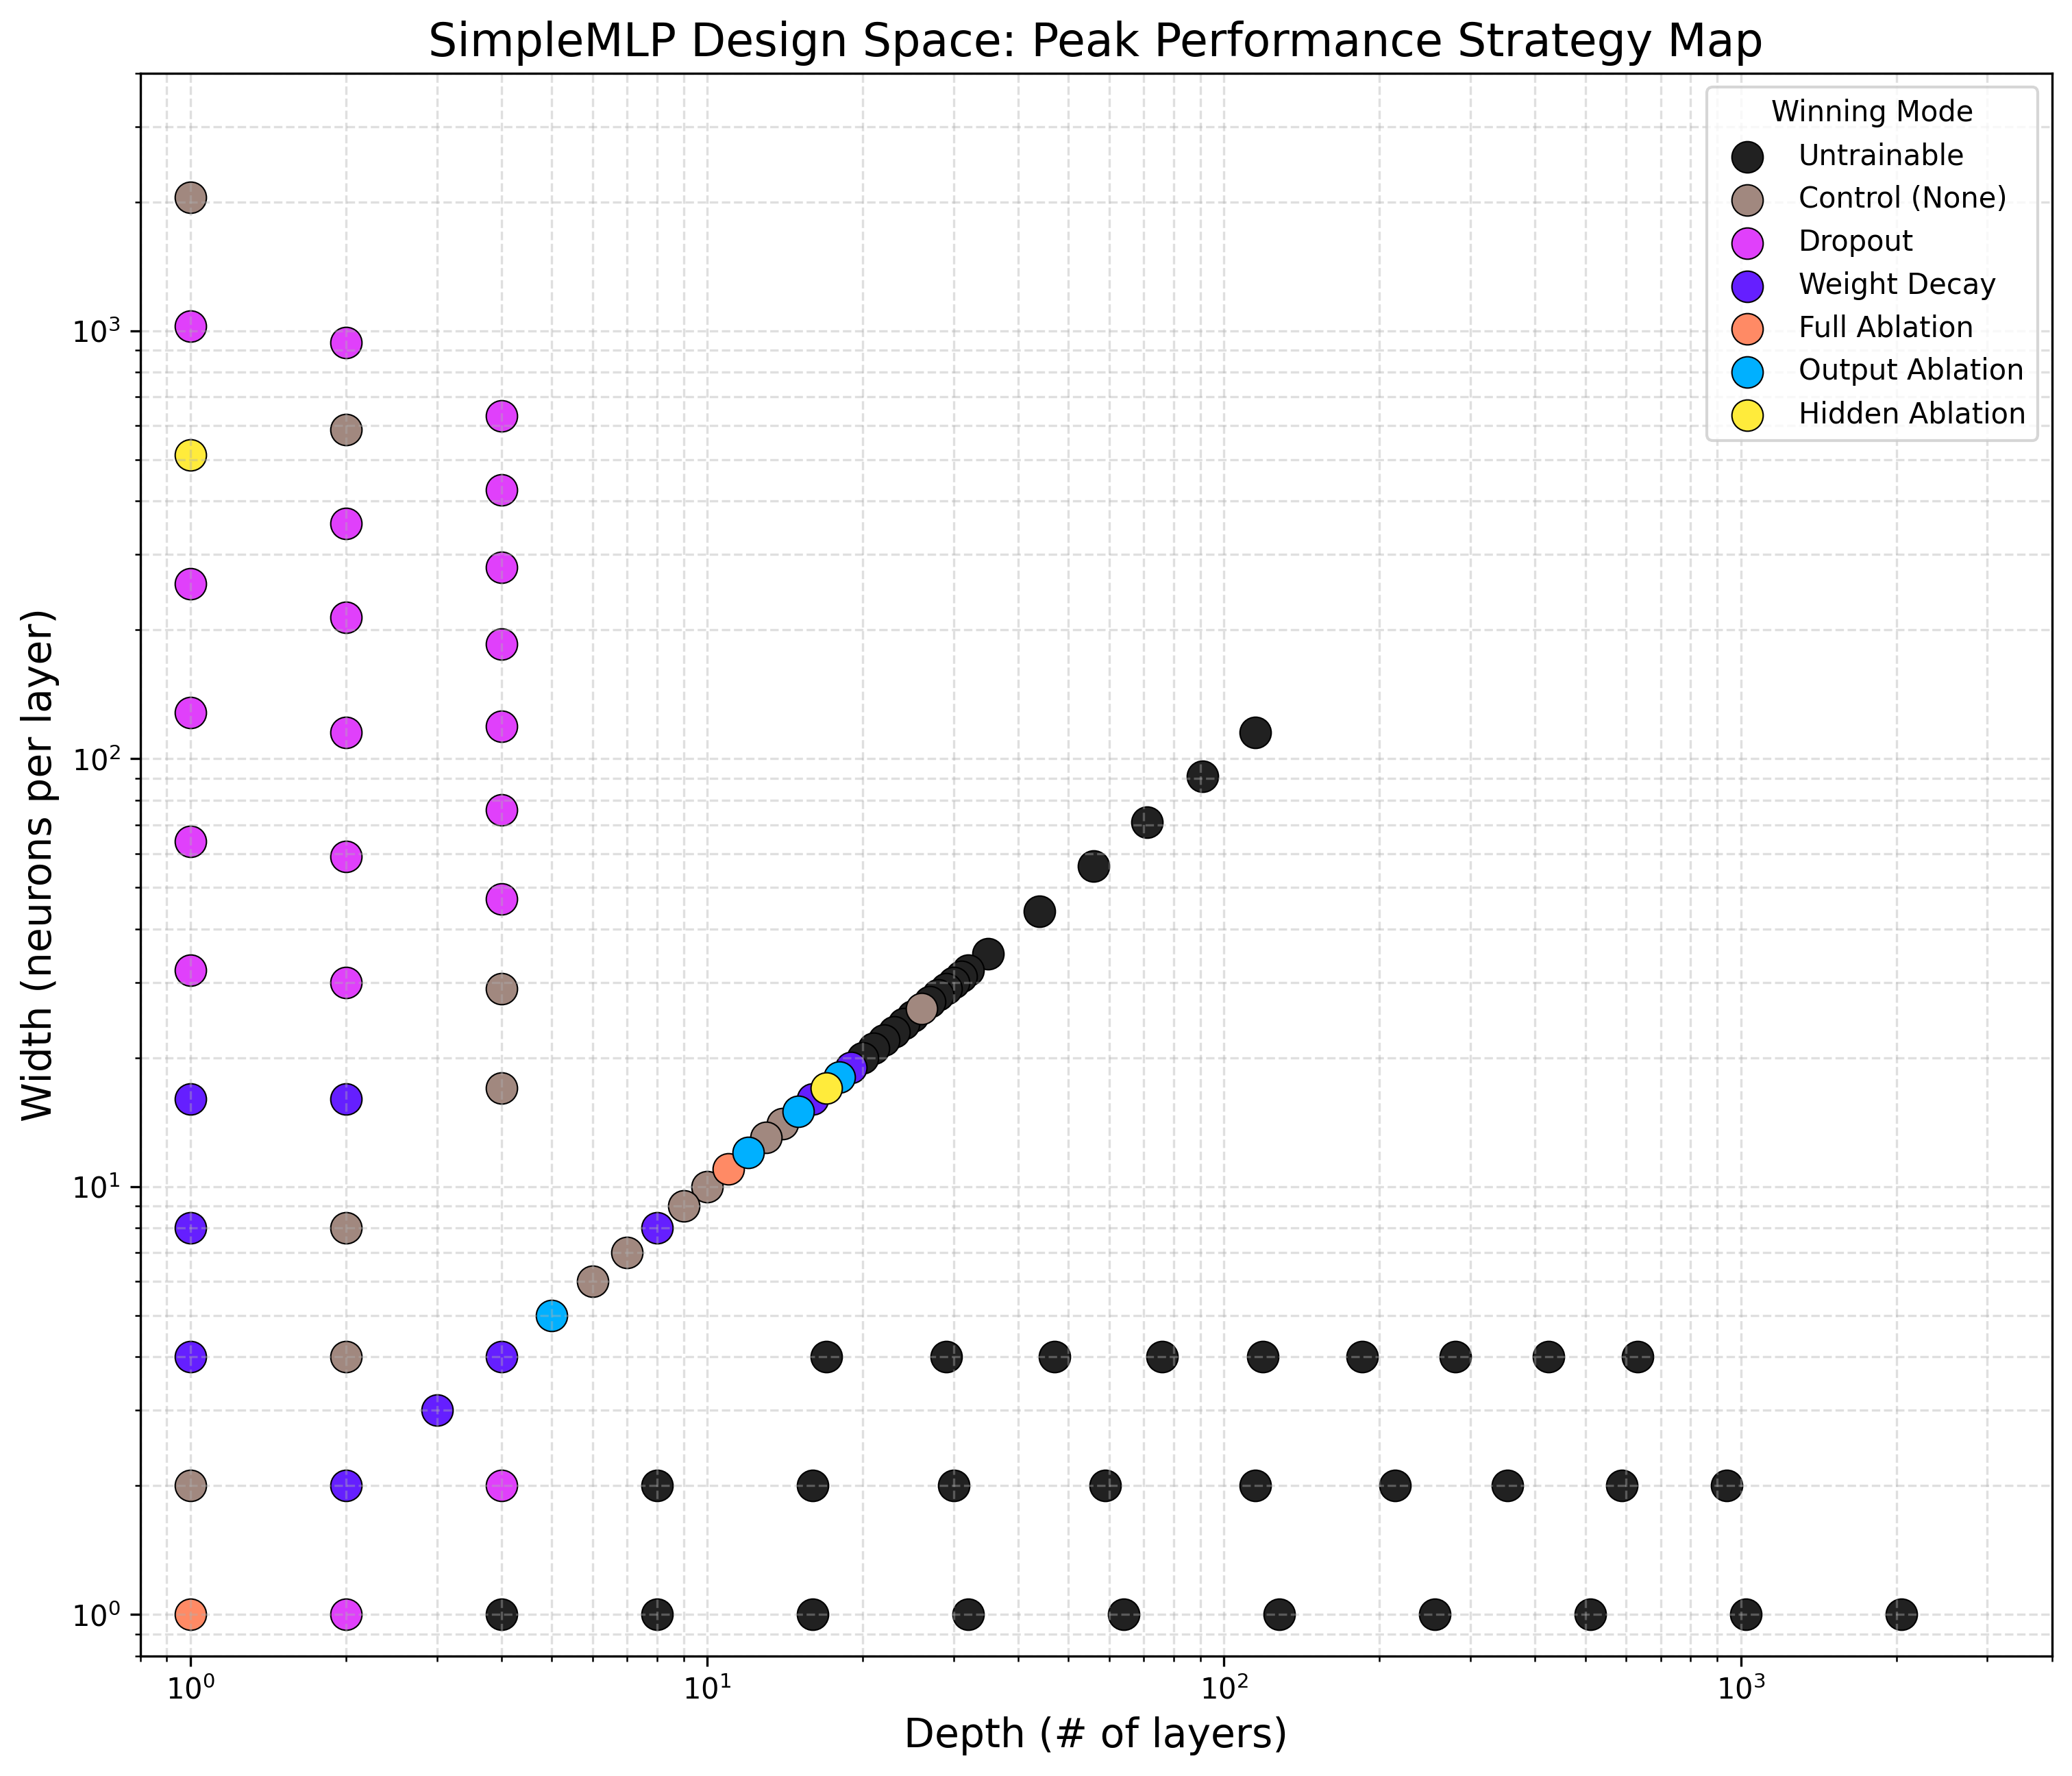
\includegraphics[width=\linewidth]{SimpleMLP_Heatmap_Winning_Strategy.png}
\caption{Winning strategies across the SimpleMLP design space. Measured by the highest score from all trials per ablation type. Note that ablation techniques demonstrated utility in training degenerate or resource constrained network configurations. The single ``win'' of the \texttt{hidden} ablation strategy in the \texttt{(18*18)} architecture stands out as an example of how persistent, random LKG ablation potentially acts as an escape mechanism from local optima.}
\label{fig:heatmap_winning}
\end{figure}

The key insight from this regime is that PSA is not a universally applicable \textit{regularizer}. Its effectiveness is contingent on the existence of network redundancy in simplistic MLP architectures. When that redundancy is unavailable in an optimally sized model, PSA's ``blind damage'' is no longer a nudge towards a more robust solution but a direct impediment to the network's ability to learn.

This presents an interesting avenue of future research on its own: detecting optimal network configurations by comparing the baseline techniques to the rate of harm that the PSA techniques are able to inflict.

\subsection{Regime III: Chaotic Optimization in Low Capacity, Unstable Models}

The most surprising results of our study emerge in a regime defined by architectural instability and reduced parametric capacity. This region (Fig. \ref{fig:regime_map}, blue points) consists of models that are on the verge of the ``Gradient Cliff'', either too deep for back-propagation due to vanishing gradients (e.g., \verb|18*18|), or so small that they lack any representational redundancy (e.g., \verb|4*4|, \verb|1*2|). Conventional gradient-based training fails in these pathological configurations, but the violent, non-gradient-based intervention of PSA seems to become a strikingly effective - albeit chaotic - optimization method.

\begin{figure}[ht]
\centering
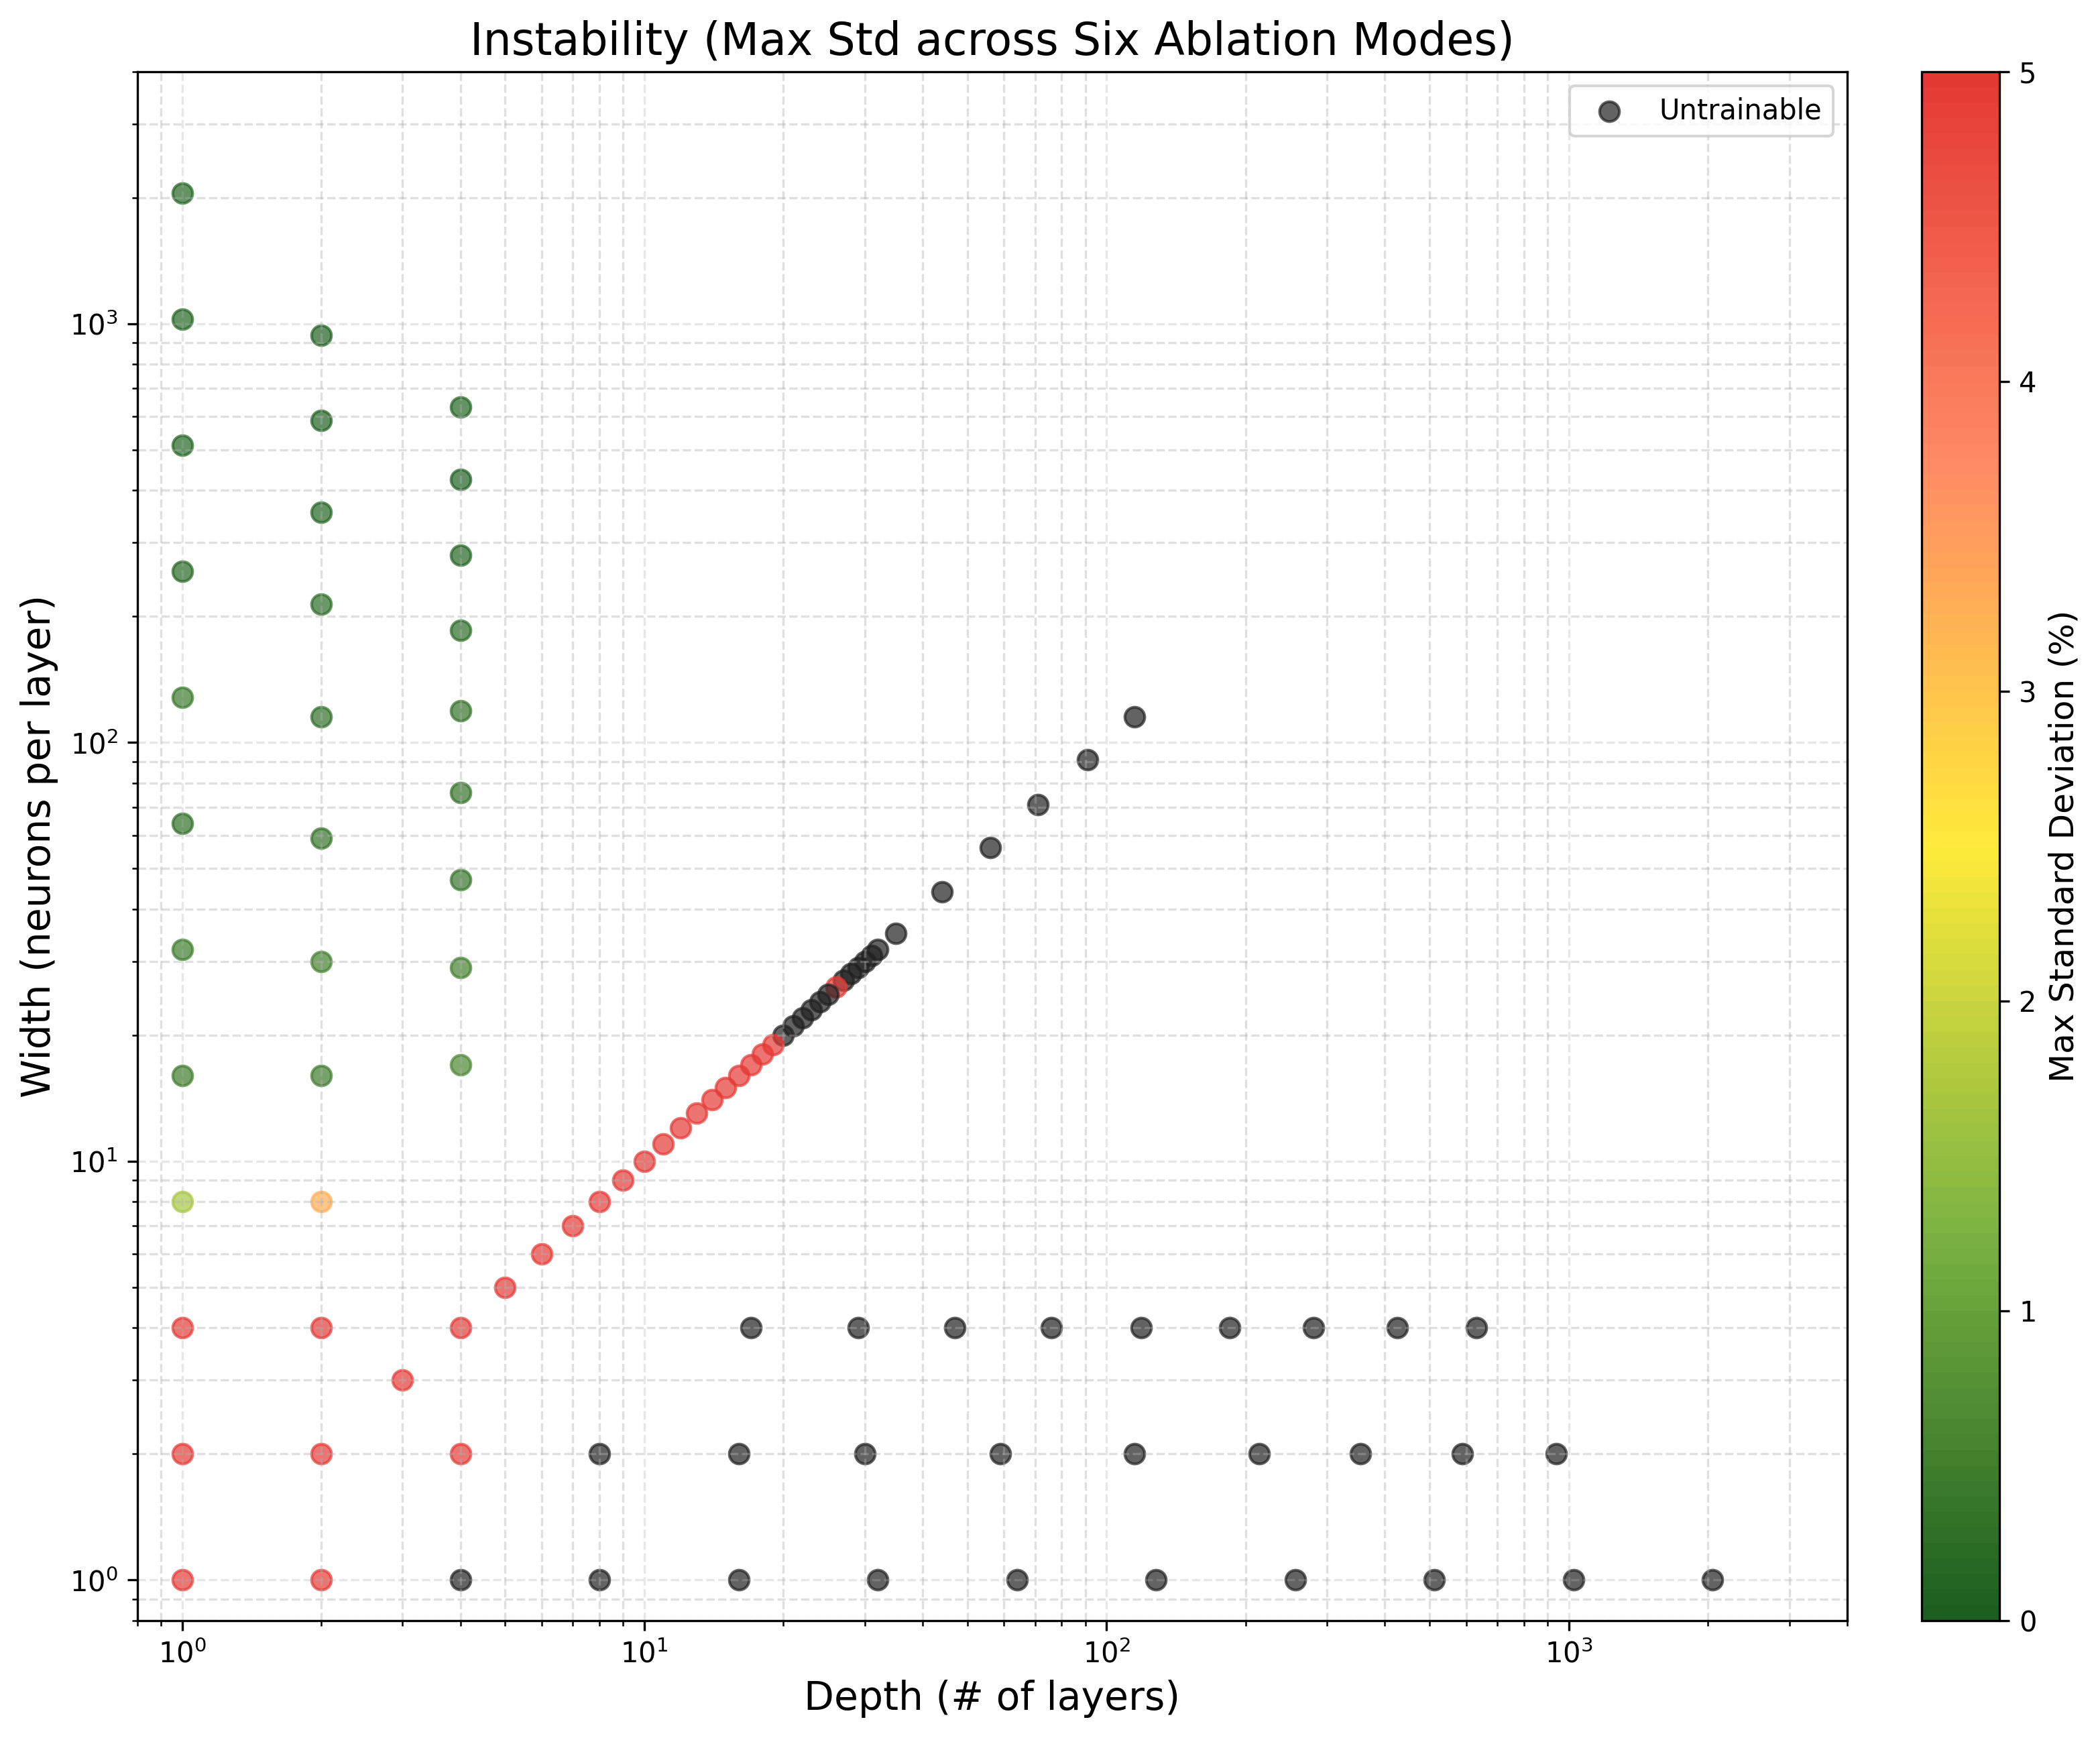
\includegraphics[width=\linewidth]{SimpleMLP_Heatmap_Instability.png}
\caption{Instability across the SimpleMLP design space, measured by the maximum standard deviation observed across the six training modes. The bright red diagonal band, corresponding to the Chaotic Optimization regime, highlights extreme performance variance, where PSA methods can induce high-scoring outliers even as baselines consistently fail. Black represents completely untrainable architectural failures.}
\label{fig:heatmap_instability}
\end{figure}

The defining characteristic of this regime is a dramatic divergence in ``uplifting'' behavior of ablative over baseline methods. As shown in the ``Baseline Performance'' map (Fig. \ref{fig:heatmap_baseline}), the \verb|none| (Control) and other traditional regularization models in this area consistently fail, yielding accuracies near the ZeroR of the validation dataset ($\sim$11.02\%); trapped in a poor local minima converged on simply guessing the validation dataset's single largest MNIST class, a state that \verb|dropout| and \verb|decay| are demonstrably unable to rescue them from.

\begin{figure}[ht]
\centering
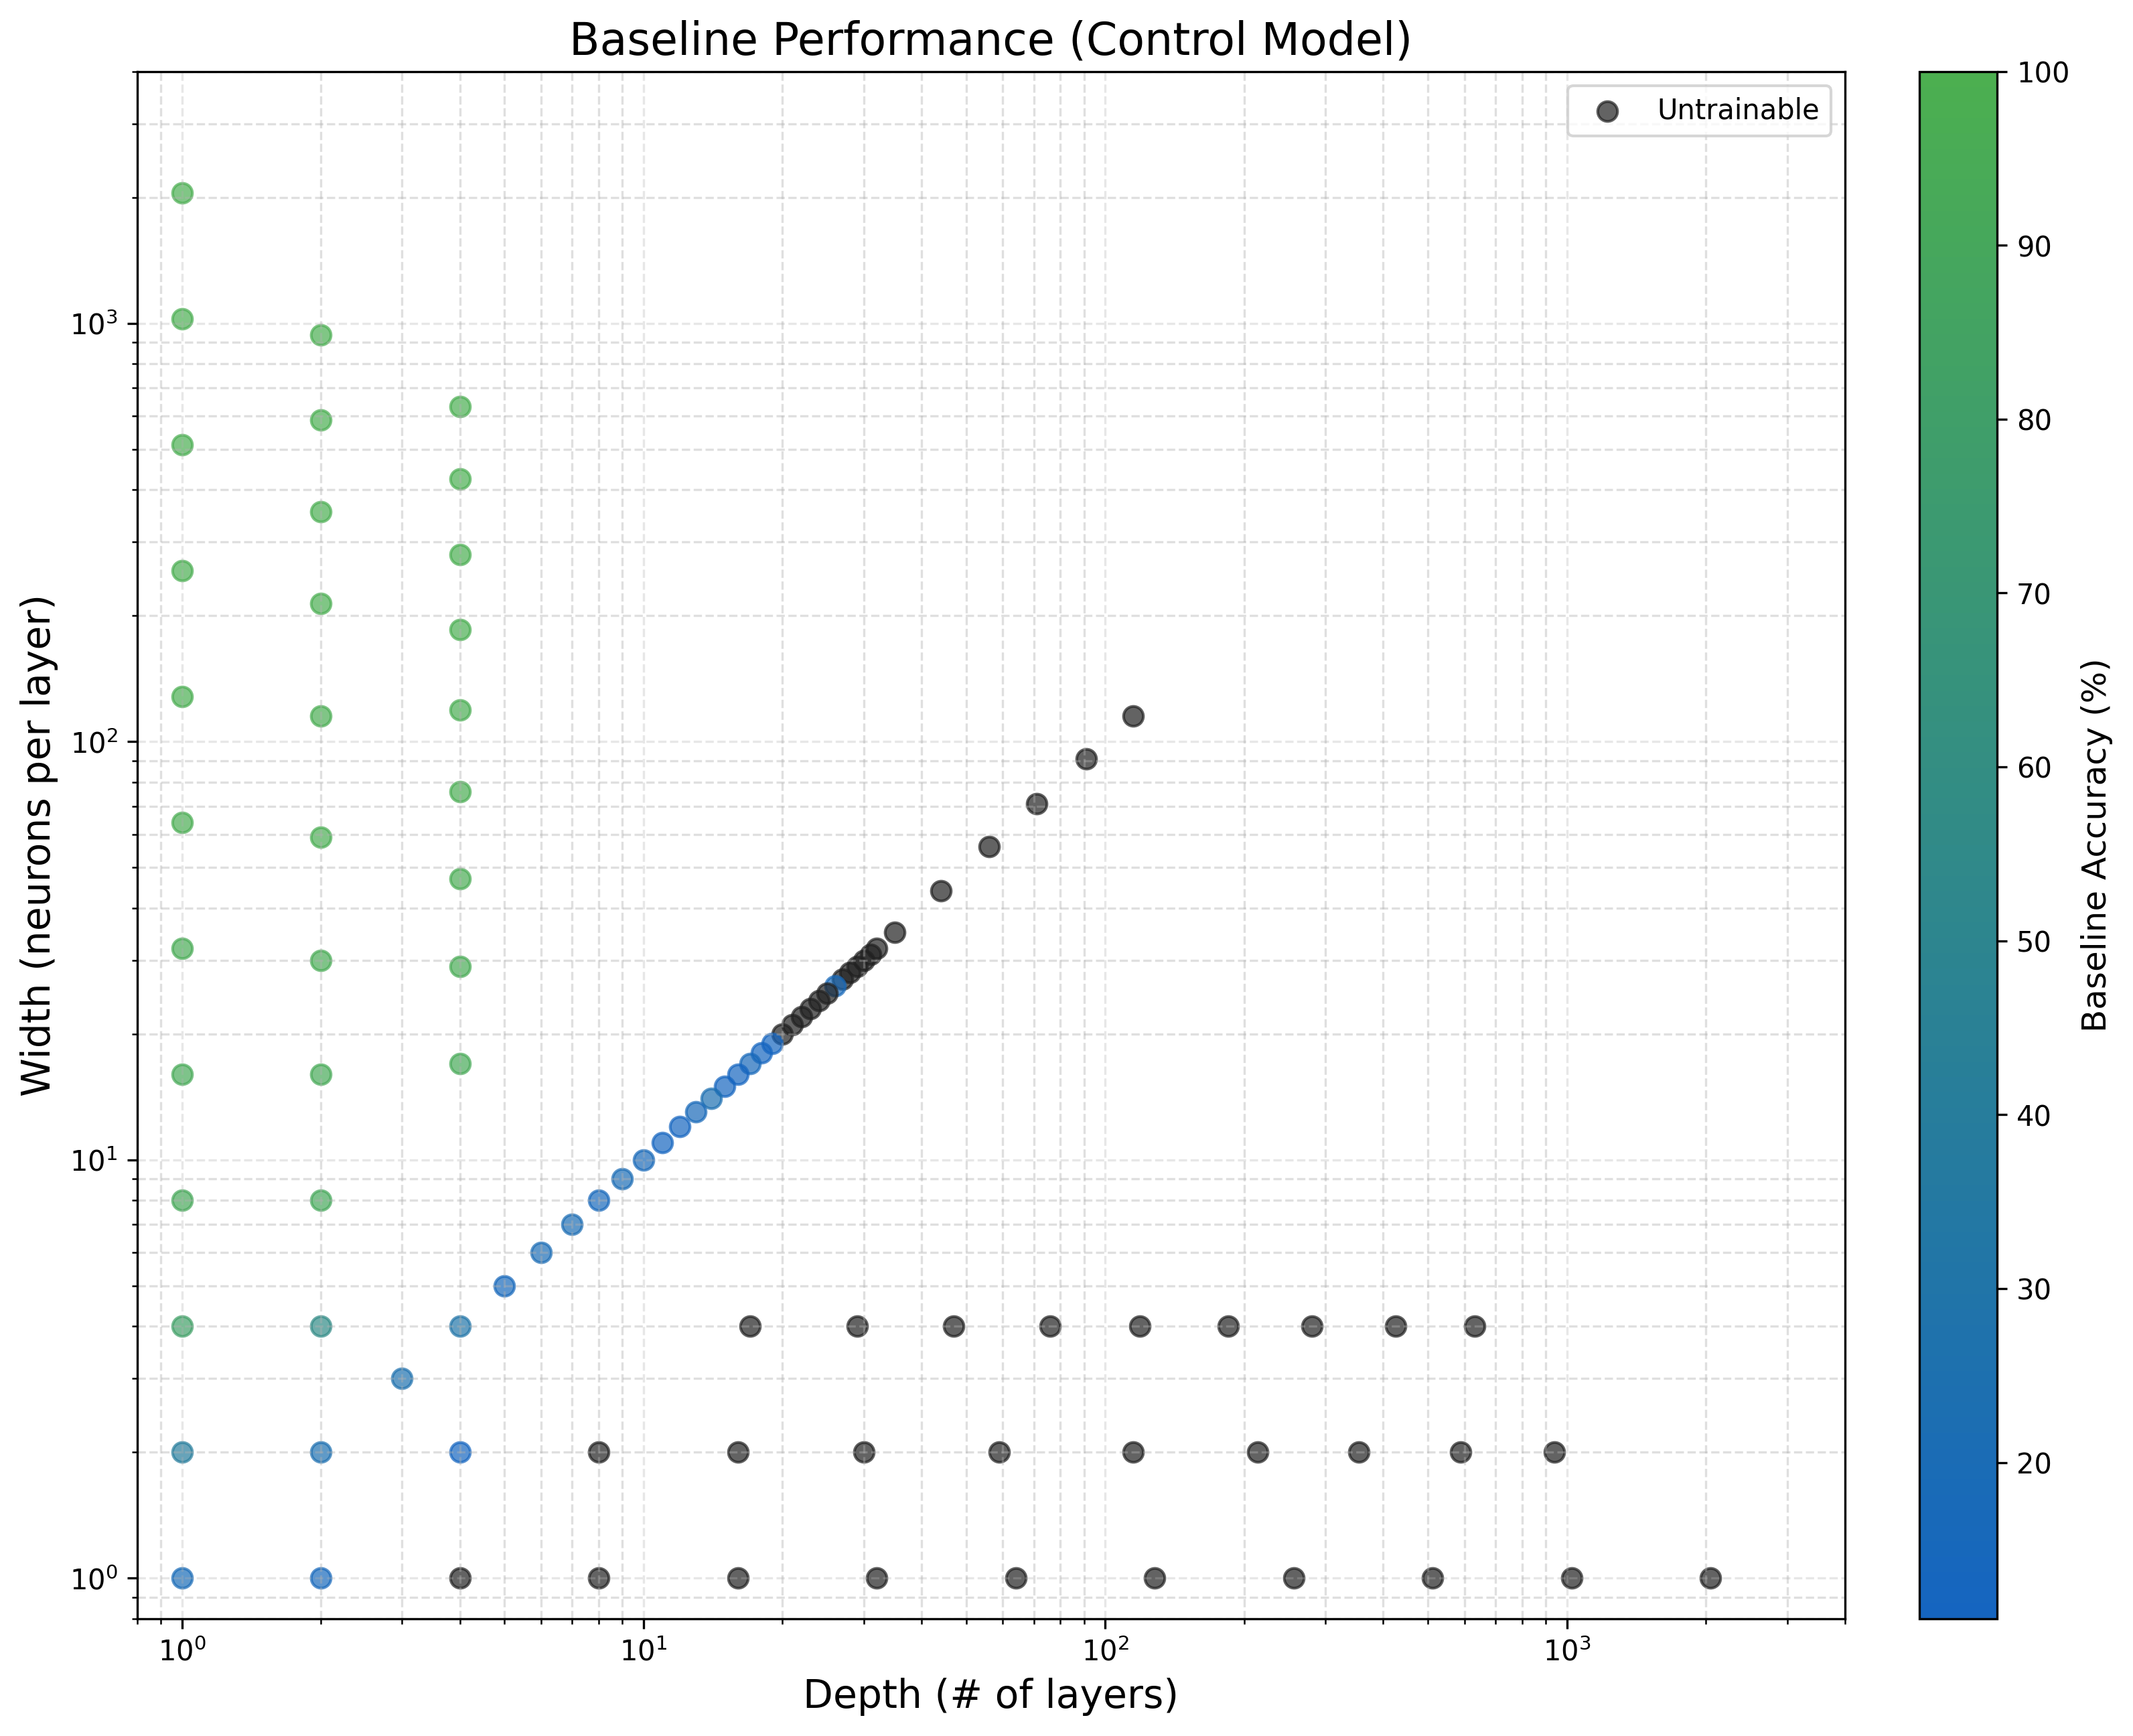
\includegraphics[width=\linewidth]{SimpleMLP_Heatmap_Baseline_Performance.png}
\caption{Baseline performance heatmap across the SimpleMLP design space. Architectures with depth $\geq$ $\sim$21 or utilizing degenerately narrow widths are untrainable across all ablation modes. These boundaries are a manifestation of the Vanishing Gradient Problem.}
\label{fig:heatmap_baseline}
\end{figure}

In positive contrast, the ``Ablation Effects'' map (Fig. \ref{fig:heatmap_ablation_effects}) reveals this same region as the only area where PSA is \textit{consistently beneficial}. (green). The ``Instability'' map (Fig. \ref{fig:heatmap_instability}) provides valuable insight: this regime exhibits the highest training variance (bright red), indicating that while many PSA trials may fail, some achieve dramatically successful outcomes. This supports our hypothesis that PSA acts as a /textbf{stochastic kick}, allowing the optimizer to escape traditionally intractable local optima.

\begin{figure}[ht]
\centering
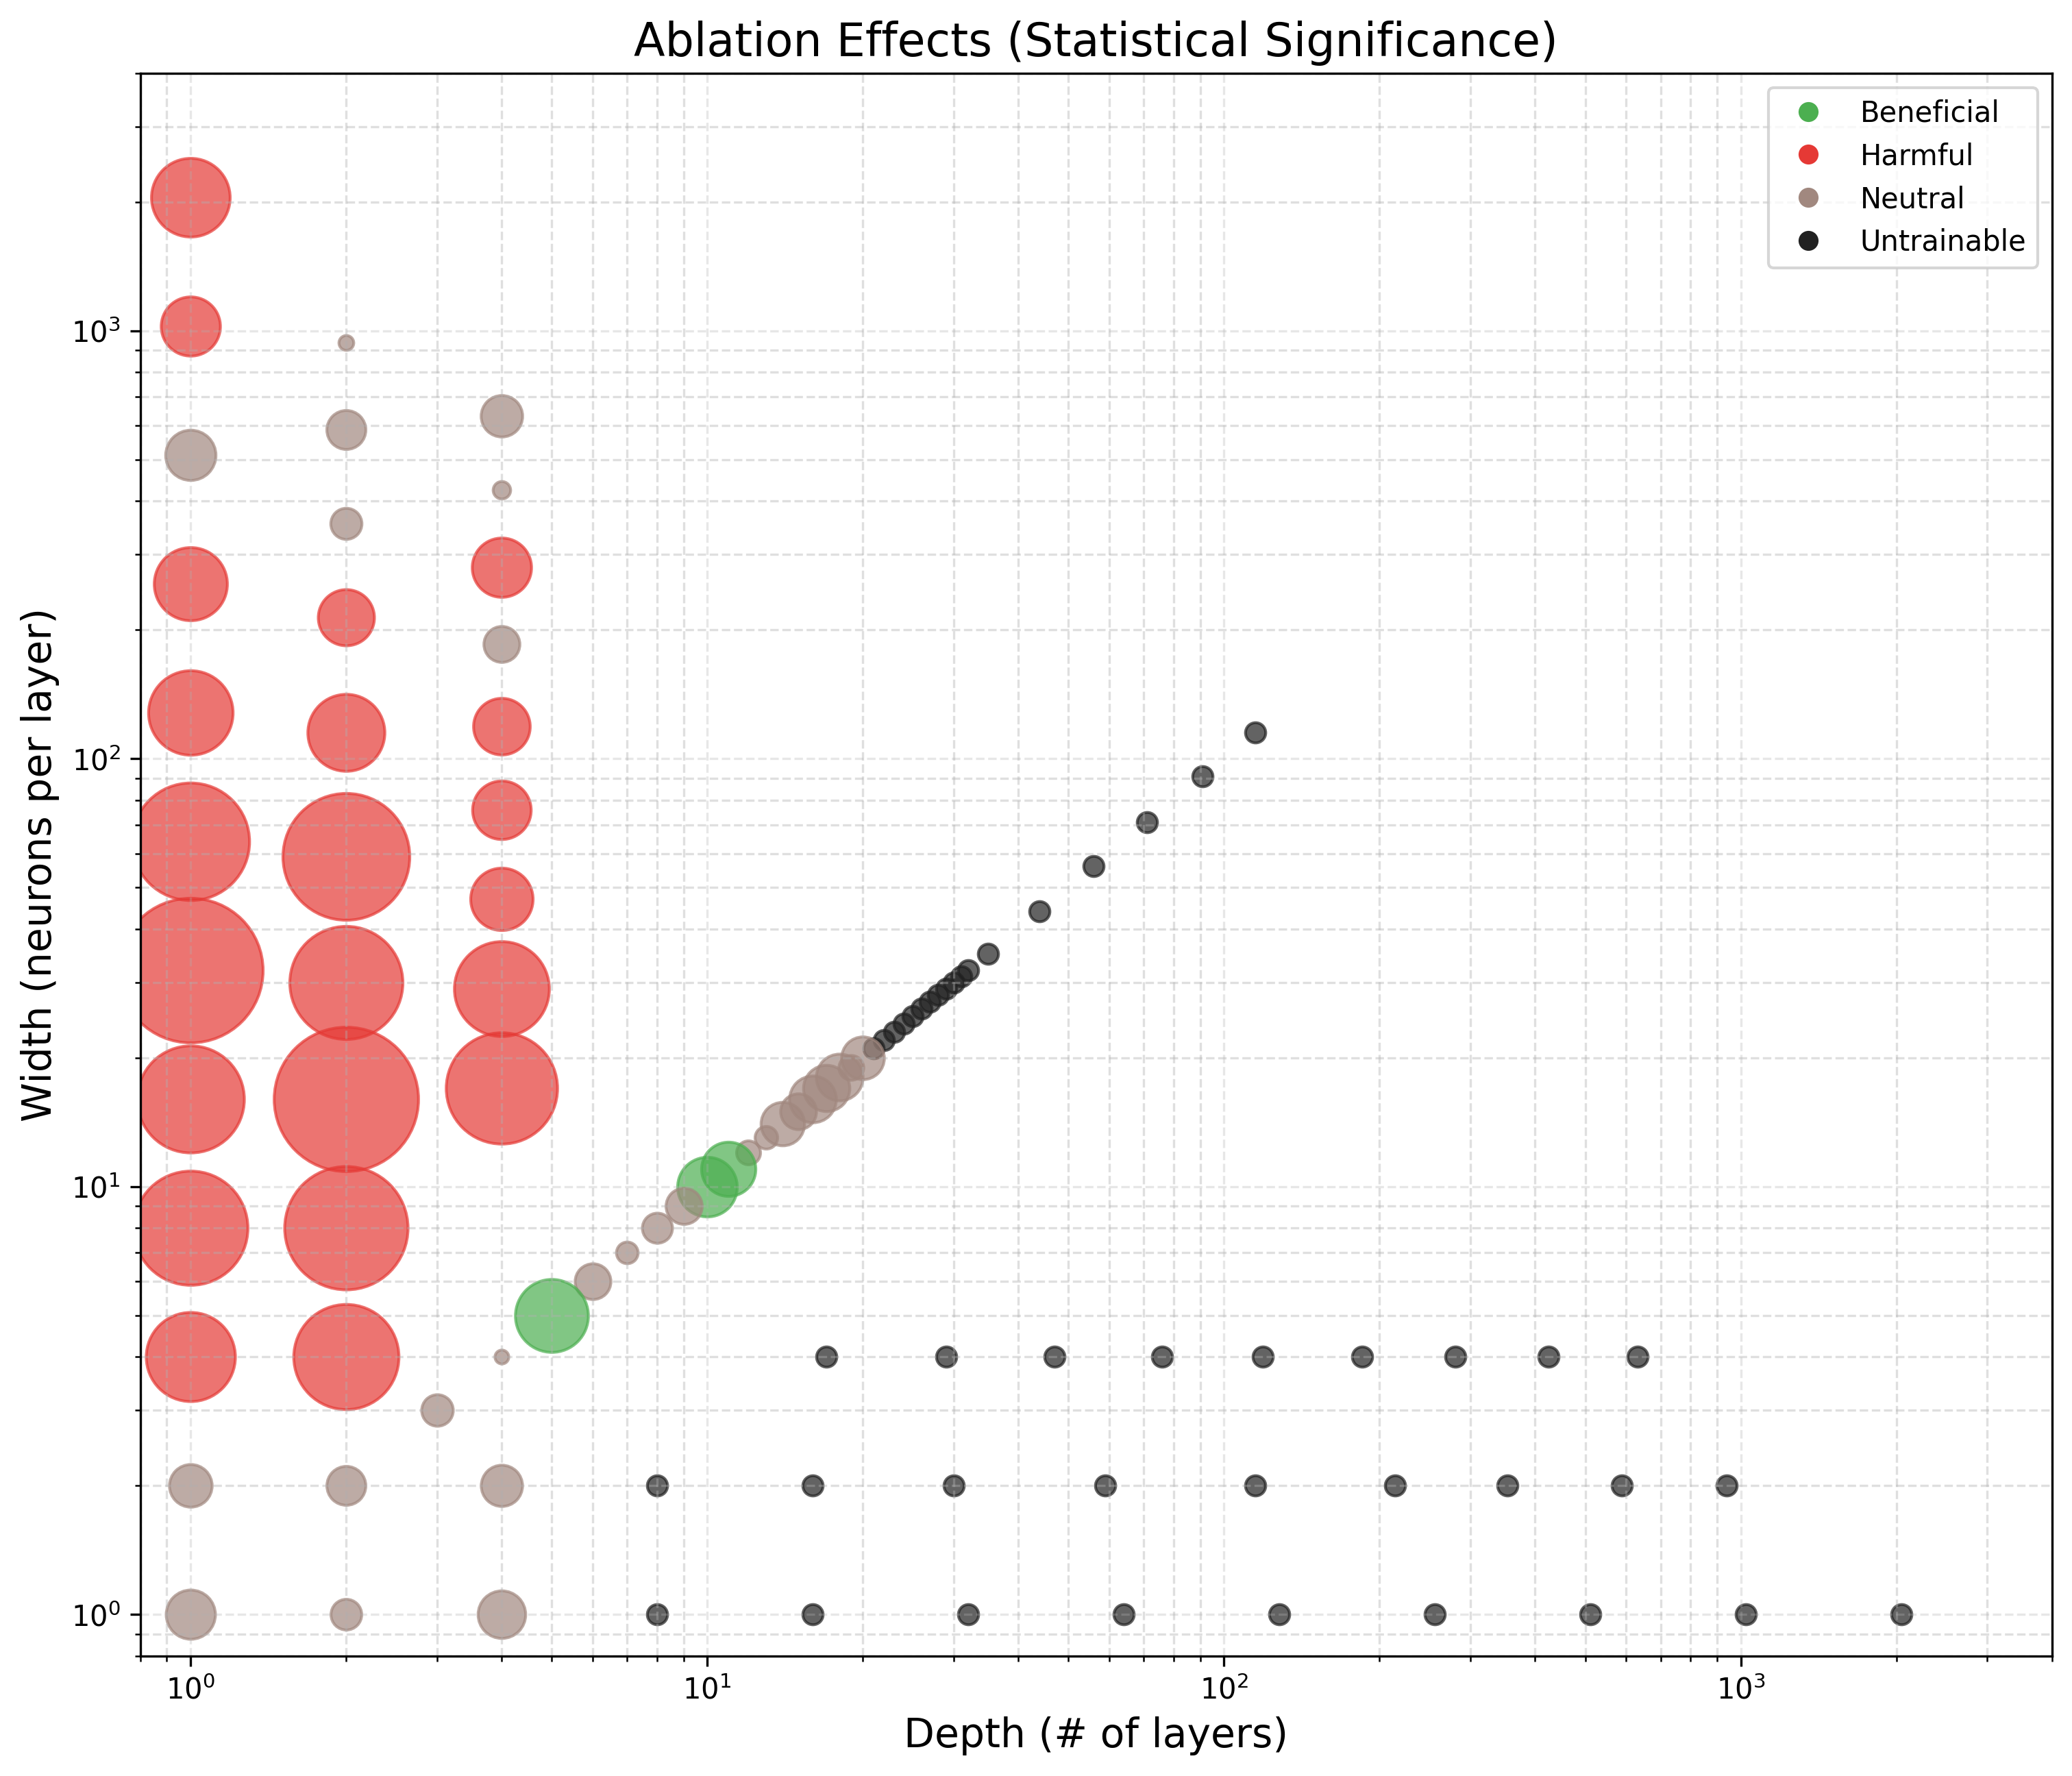
\includegraphics[width=\linewidth]{SimpleMLP_Heatmap_Ablation_Effects.png}
\caption{Ablation effects (beneficial or harmful) across the SimpleMLP design space. In the trainable models there are clear regimes where ablation either is beneficial, harmful, or indistinguishable from the baseline.}
\label{fig:heatmap_ablation_effects}
\end{figure}

A powerful example is the \texttt{19*19} architecture with \texttt{21,955} parameters. Table \ref{tab:19x19_results} shows a total failure of the baseline methods (e.g., a maximum of 11.02\% over all 10 trials). However, the \verb|hidden| and \verb|output| PSA modes produce massive improvements in peak performance, at 47.14\% and 63.12\% respectively.

\begin{table}[h!]
\centering
\caption{Performance Summary for the \texttt{19*19} Architecture\\ \texttt{21,955} Parameters (n=10).}
\label{tab:19x19_results}
\begin{tabular}{lcccc}
\toprule
\textbf{Mode} & \textbf{Mean} & \textbf{Std} & \textbf{Min} & \textbf{Max} \\
\midrule
None    & 10.34\% & 0.54\% & 9.72\% & 11.02\% \\
Decay   & 10.21\% & 0.91\% & 8.65\% & 11.02\% \\
Dropout & 10.24\% & 0.51\% & 9.72\% & 11.02\% \\
Full    & 10.45\% & 0.57\% & 9.72\% & 11.02\% \\
Hidden  & 13.80\% & 11.12\% & 9.72\% & 47.14\% \\
Output  & \textbf{19.08\%} & 15.45\% & 10.10\% & \textbf{63.12\%} \\
\bottomrule
\end{tabular}
\end{table}

Critically, the separation of PSA into three different modes allows us to disentangle the effects of ablative placement and method. The ``Winning Strategy Map'' (Fig. \ref{fig:heatmap_winning}) shows that no single PSA mode dominates this chaotic regime; instead, the optimal strategy depends on the specific architectural pathology.

\begin{itemize}
    \item \textbf{Hidden Ablation (Full Neuron Ablation):} For the deep but unstable square model \texttt{18*18}, \textbf{Hidden} ablation was the most effective strategy. This method performs a \textit{full neuron ablation} by zeroing both the bias, incoming, and outgoing weights of randomly chosen hidden neurons. It suggests that for networks trapped by the Vanishing Gradient Problem, a more aggressive stochastic ``kick'' may fundamentally alter the network's functional pathways and escape the poor local minimum.

    \item \textbf{Full \& Output Ablation (Partial Ablations):} In contrast, for extremely small, resource-starved models such as \texttt{4*4} and \texttt{1*2}, the winning strategies were \textbf{Full} and \textbf{Output} ablation. These methods use a less destructive \textit{partial ablation} (zeroing only incoming weights and the bias). This finding suggests that when a model has very few parameters to begin with, a more targeted perturbation is more effective. Note that the \verb|output| is the most aggressive and chaotic of the three modes due to directly zeroing the weights of output logits.
\end{itemize}

This regime provides the strongest evidence for the non-regularization utility of PSA. It demonstrates that blind, persistent damage can serve as a powerful tool for online stochastic optimization, offering a lifeline to models that might be otherwise untrainable with standard gradient-based methods.

Our findings around the ``stochastic kick'' behavior, where a random perturbation might dramatically improve an otherwise failing training optimization process, seems conceptually similar to the effectiveness of random search for hyper-parameter optimization, often outperforming grid search in high-dimensional, non-convex problem spaces \cite{b7}.

\subsection{Regime IV: Architectural Failure in Zero Capacity, Unstable Models}

The final regime encompasses architectures that are \textit{fundamentally untrainable}: where the choice of training strategy becomes irrelevant. Our systematic exploration of the design space was designed to map the precise boundary of this failure as an observable phenomenon where even the powerful stochastic kick of PSA is insufficient to rescue the model from architectural collapse.

Models in this regime (Fig. \ref{regime_map}, black points) universally fail to learn, with all six training modes stalling at an accuracy of approximately 11.02\%. This value is the empirically measured majority class baseline (ZeroR) for our 10,000-sample validation set, confirming a total failure to learn from input features. This failure is attributable to two distinct architectural pathologies: the \textit{Vanishing Gradient Problem} in excessively deep networks, and \textit{Information Bottlenecks} in degenerately narrow ones.

\subsubsection{The VGP Boundary in Square Architectures}

One of the primary goals of our study was to identify the exact depth at which a simple MLP becomes untrainable on MNIST. Our exploration of square models revealed this boundary between a depth of 20 and 21 layers.

As shown in Table \ref{tab:20v21_results}, the \texttt{20*20} architecture resides within the Chaotic Optimization regime. While its baseline methods fail, the \textbf{Full} ablation mode is able to provide a stochastic kick, achieving a peak accuracy of 20.91\%. This demonstrates that at a depth of 20, the model is on the absolute edge of failure yet remains salvageable by PSA.

The \texttt{21*21} architecture, just one layer deeper, \textit{completely fails to train}. All six training modes, including every PSA variant, fail completely, with no trial exceeding the 11.02\% baseline. The stochastic kick is no longer powerful enough to escape a loss landscape that has possibly become intractably flat due to the compounded decay of gradients through 21 successive layers, nor can the traditional regularization methods traverse the region in a meaningful way.

\begin{table}[h!]
\centering
\caption{Performance Collapse at the VGP Boundary (n=10).}
\label{tab:20v21_results}
\resizebox{\columnwidth}{!}{%
\begin{tabular}{l|cccc|cccc}
\toprule
& \multicolumn{4}{c|}{\textbf{\texttt{20*20} (Salvageable)}} & \multicolumn{4}{c}{\textbf{\texttt{21*21} (Untrainable)}} \\
\textbf{Mode} & \textbf{Mean} & \textbf{Std} & \textbf{Min} & \textbf{Max} & \textbf{Mean} & \textbf{Std} & \textbf{Min} & \textbf{Max} \\
\midrule
None & 10.39\% & 0.51\% & 9.72\% & 11.02\% & 10.46\% & 0.44\% & 10.09\% & 11.02\% \\
Decay & 10.34\% & 0.75\% & 8.65\% & 11.02\% & 10.13\% & 0.45\% & 9.72\% & 11.02\% \\
Dropout & 10.15\% & 0.46\% & 9.72\% & 11.02\% & 10.33\% & 0.47\% & 9.81\% & 11.02\% \\
Full & \textbf{11.77\%} & 3.07\% & 9.84\% & \textbf{20.91\%} & 10.51\% & 0.49\% & 9.73\% & 11.02\% \\
Hidden & 10.37\% & 0.52\% & 9.81\% & 11.02\% & 10.48\% & 0.53\% & 9.72\% & 11.02\% \\
Output & 10.66\% & 0.45\% & 10.10\%& 11.02\% & 10.82\% & 0.36\% & 10.09\% & 11.02\% \\
\bottomrule
\end{tabular}
}
\end{table}

The identification of this boundary highlights the limitations of our SimpleMLP testbed. Architectures like ResNet\cite{b8} or the more recent ResMLP\cite{b9} were designed specifically to overcome this boundary by introducing skip connections, providing uninterrupted paths for gradient flow, and enabling the training of much deeper networks.

\subsubsection{Information Bottlenecks in Deep-and-Narrow Architectures}

The second cause of architectural failure is the information bottleneck. This occurs in our ``deep-and-narrow'' configurations (e.g., L*4, L*2, L*1). While the shallowest of these, such as 1*1 and 2*1, are technically trainable (albeit with poor performance, landing them in the Chaotic Optimization regime), they quickly become untrainable as depth increases.

It is self-evident that collapsing the 784-pixel input of the MNIST dataset into a 1-neuron wide set of layers irrevocably destroys critical spatial data, and these maximally degenerate cases were included not just for the sake of ``completeness'' but to identify the boundaries where any possible learning \textit{stops}, especially when compared to other deep-and-narrow yet slightly wider topologies.

\subsection{Empirical Convergence Dynamics}

By examining the detailed CloudWatch logs from our wide-scale run of 5,880 trials we extracted the temporal pattern of the validation accuracy's improvement, stalling, and failures for each of the 588 experimental configurations across all 10 of their 100 meta-loop trial runs.

While final peak accuracy may reveal the ultimate effectiveness of a given training strategy, the temporal pattern of each trial offers deep insights into the underlying optimization dynamics, allowing us to directly observe the stability and convergence properties of each combination of architecture and training technique. This detailed data, visualized for several key architectures in Figure~\ref{fig:convergence_plots}, provides clear evidence for the different roles played by baseline and PSA methods and empirical support for our reasoning about classification into four training regimes.

\subsubsection{Stable Convergence vs. Exploratory Volatility}

\begin{figure*}[ht]
    \centering
    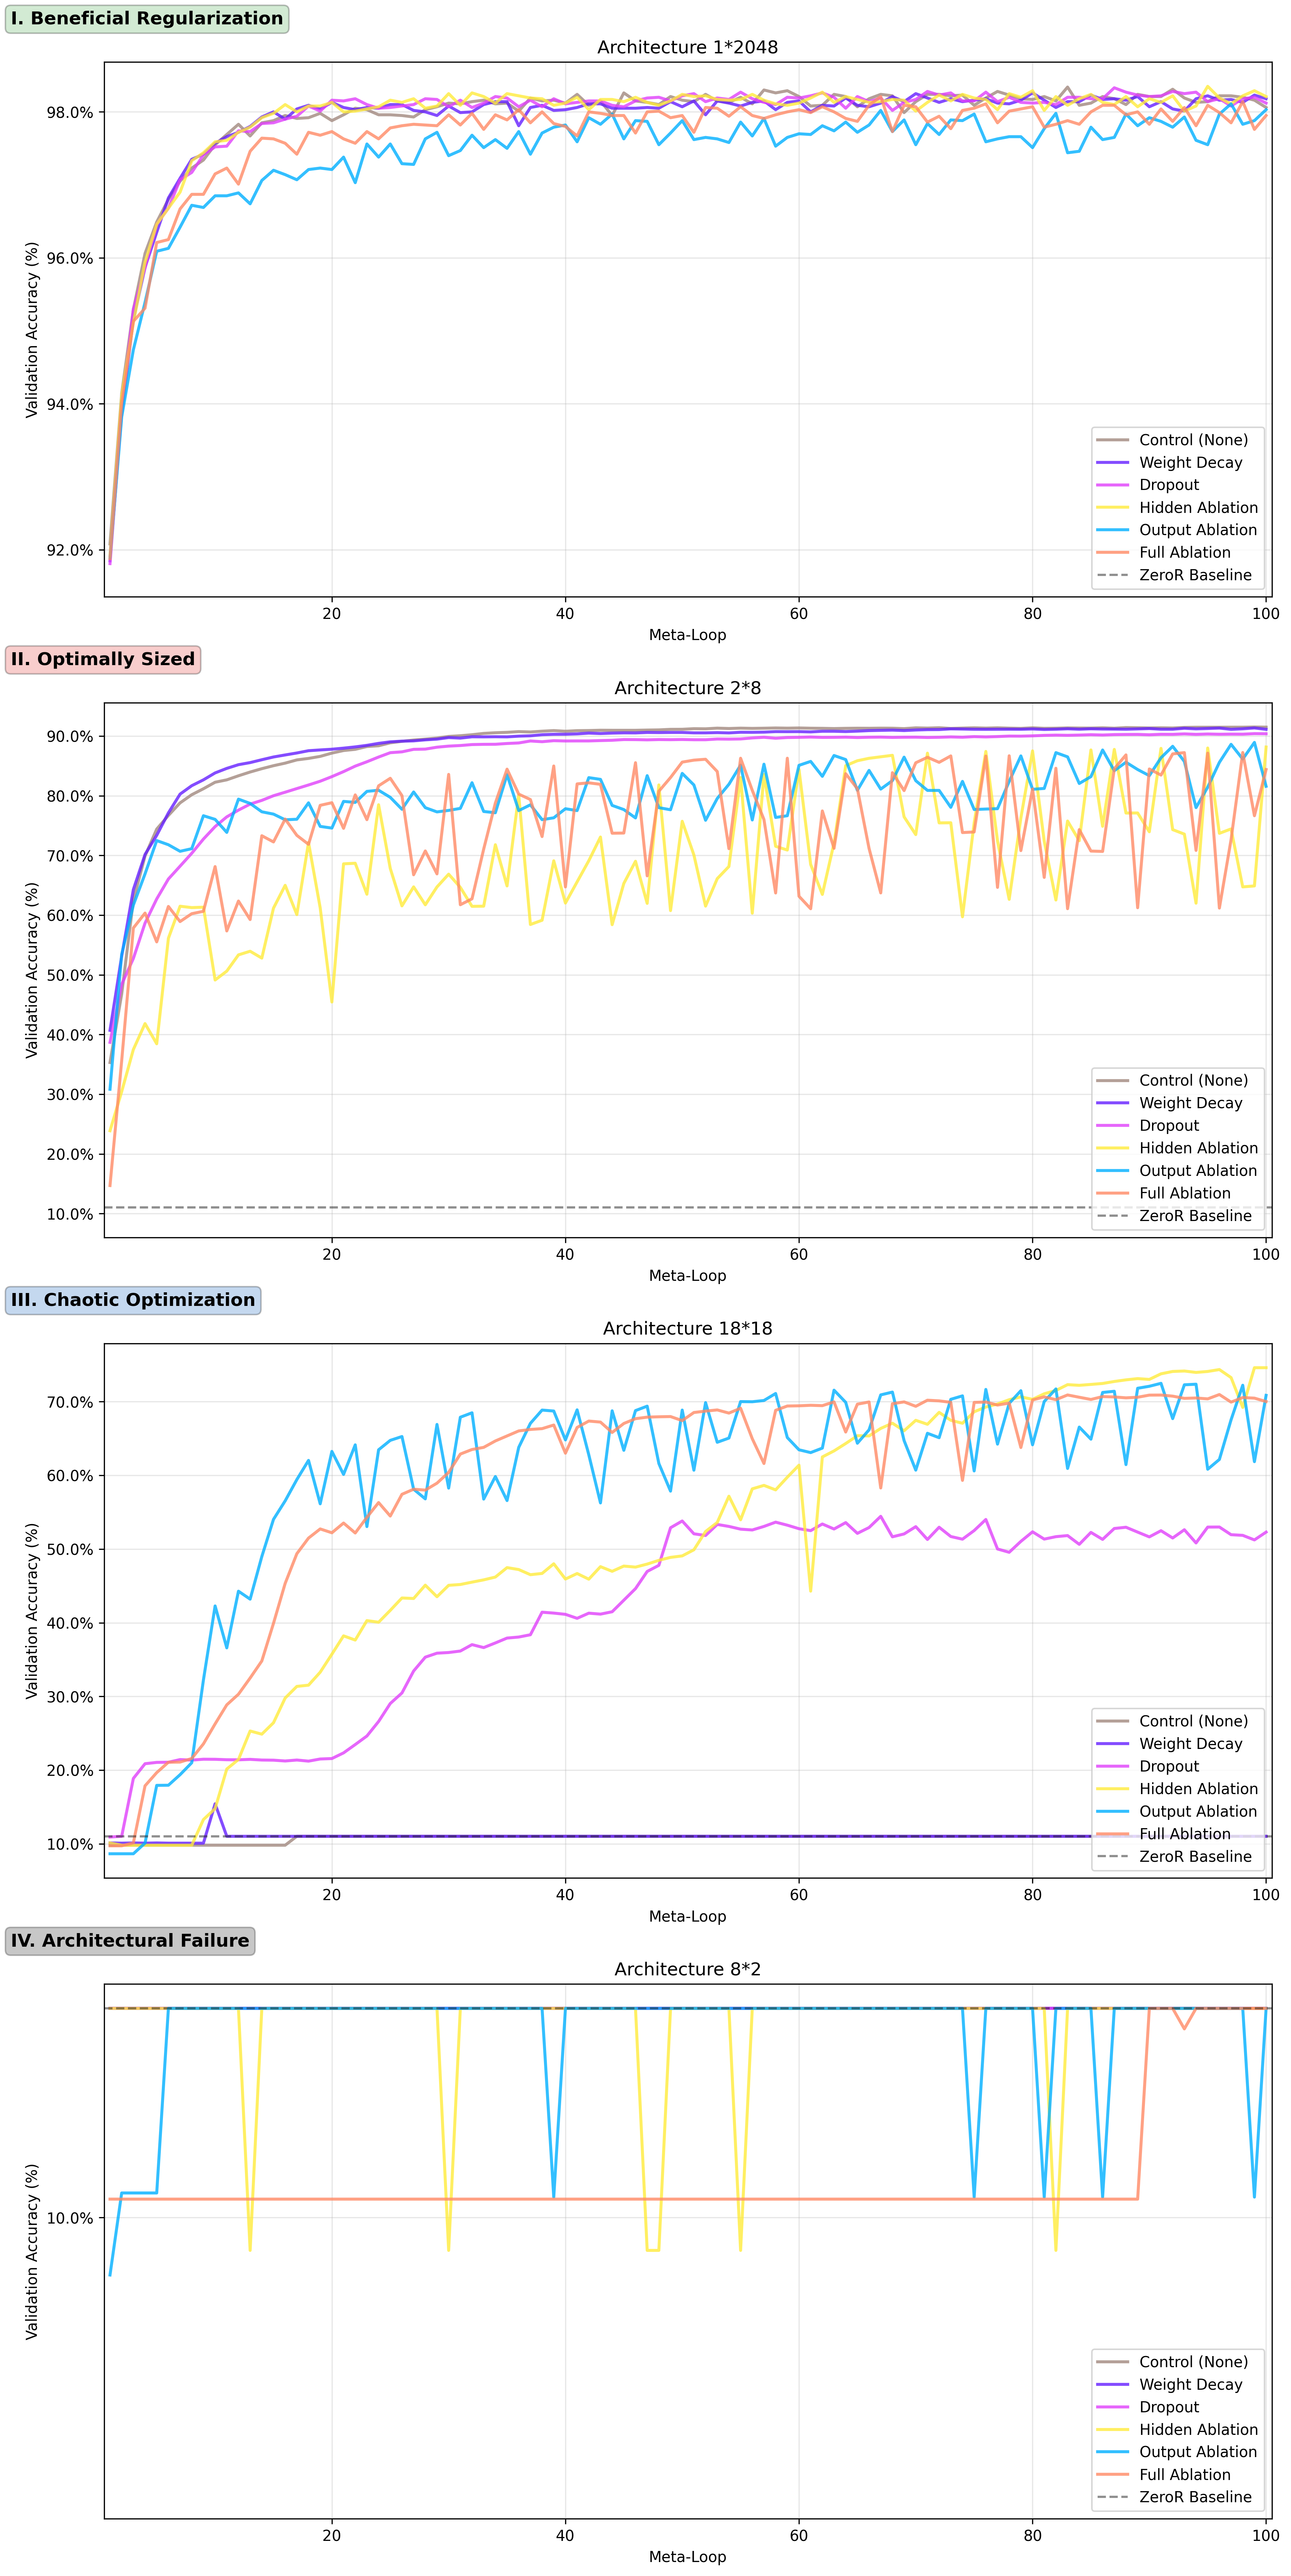
\includegraphics[width=\columnwidth]{SimpleMLP_Plot_Convergence.png}
    \caption{Convergence dynamics across training regimes, plotting per-``meta-loop'' validation accuracy for all 10 trials of each mode, with the peak performing trials for a given architecture plotted.}
    \label{fig:convergence_plots}
\end{figure*}

In stable architectures, such as the over-parameterized \texttt{1*2048} model (Figure \ref{fig:convergence_plots}, Top), all six training modes exhibit smooth and rapid convergence. The baseline methods (\verb|none|, \verb|decay|, \verb|dropout|) quickly achieve a high-performance plateau. The PSA modes also converge to a similar performance ceiling over a longer time horizon, still gaining minor improvements even up to the final meta-loops, demonstrating both the inherent redundancy of the larger models allowing consistent recovery from the stochastic ablation, and a need to do further trials beyond 100 meta-loops to measure how far continued PSA-driven improvements might extend during training.

The dynamics diverge dramatically in the \textbf{Chaotic Optimization} regime. For the \texttt{18*18} architecture (Figure \ref{fig:convergence_plots}, Second from Bottom), the baseline methods are completely unable to escape a quickly identified, poor local minimum: flat-lining at the ZeroR baseline for all 100 meta-loops. The learning curves for the PSA methods, however, are extremely volatile. This is the direct empirical signature of the ``Frustration Engine'' at work: each point represents a recovery attempt from a newly damaged state. Many attempts fail, resulting in performance drops back towards the baseline. However, this high-variance search process seems to allow the optimizer to explore a much wider solution space. We believe it is this chaotic exploration that enables PSA to discover optimization pathways that lead to significant performance breakthroughs, reaching accuracies far beyond what the stable, gradient-based methods achieve on their own.

\subsubsection{Stochastic Exploration Cost and Benefit}

This volatility represents the inherent ``cost of exploration'' in the PSA paradigm: many candidate models are ultimately discarded. However, our analysis reveals that this is a central mechanism of the method's utility in unstable architectures, as the repeated ``kicks'' from a disadvantaged state are precisely what prevent the optimizer from getting permanently trapped. The success of PSA in the Chaotic Optimization regime demonstrates that for certain pathological loss landscapes, abandoning monotonic convergence in favor of a volatile, persistent search is possibly an effective, albeit lengthy, optimization strategy.

It also leaves the door open for post-regularization ``kicks'' into nearby but valuable optima once a traditional regularization technique like Dropout has done all it can, and this will be an avenue of further research.

\section{Discussion and Limitations}
The four regimes identified in our results provide a unified theory for the behavior of PSA on simplistic MLPs. Its utility is an emergent property represented within a two dimensional phase space of optimization opportunities across the non-linear axes of parametric capacity and architectural stability. The ``gradient cliff'' encountered in Regime IV, however, places a hard limitation on this initial study. We cannot know how PSA affects truly deep networks if the baseline architecture itself is untrainable.

Our exhaustive study reveals that the primary utility of Persistent Stochastic Ablation is not as a regularizer, but as a surprisingly powerful tool for stochastic optimization. The most significant finding of this work is the emergence of the ``Chaotic Optimization'' regime, where the random, non-gradient-based ``kick'' from PSA provides a lifeline to architecturally unstable models.

For these pathological networks, trapped in poor local minima by the Vanishing Gradient Problem or degenerate Information Bottlenecks, PSA provides a method capable of inducing meaningful learning, outperforming conventional baselines like Dropout and Weight Decay. While PSA can confer a minor regularizing effect in stable, over-parameterized models, this benefit is neither statistically significant nor competitive with established techniques over the training intervals we observed (100 meta-loops).

We find that PSA's currently demonstable value lies not in refining well-behaved models, but in rescuing otherwise untrainable ones, possibly positioning PSA as a novel mechanism for exploring intractable loss landscapes and motivating our future work in applying this paradigm to more complex architectures where optimization challenges persist.

Key limitations of this initial study include:
\begin{itemize}
    \item \textbf{Architectural Weakness:} The study was confined to simple MLPs, which lack modern components like residual connections (as in ResNet)\cite{b8} or normalization layers (like Batch Norm)\cite{b10}. The observed efficacy of PSA might be entirely different in more complex and robust architectures, or disappear altogether.
    \item \textbf{Single, Simple Dataset:} All experiments were conducted on MNIST. While useful for a proof-of-concept, its low complexity is not representative of the challenges posed by more complex, real-world datasets (e.g., CIFAR-100, ImageNet). The benefits of PSA could be magnified, diminished, or altered on more difficult problems.
    \item \textbf{Fixed Ablation Strategy:} The PSA mechanism was fixed to ablating exactly one neuron per meta-loop. The effects could change dramatically with different strategies, such as ablating a percentage of neurons, targeting specific layers, or adaptively varying the rate of ablation over the course of training.
    \item \textbf{Fixed Optimizer Hyperparameters:} The underlying optimization algorithm (e.g., AdamW\cite{b11}) and its hyperparameters (e.g., learning rate) were held constant across the vastly different architectures. It is possible that some of the ``Architectural Failures'' could have been mitigated with architecture-specific tuning, potentially altering the winning ablation mode in some regimes.
    \item \textbf{Limited Training Intervals:} We trained each model for only 100 meta-loops, and while existing regularization techniques like Dropout and Weight Decay quickly converged with the first 30-75\% of the training intervals, several PSA modes were still finding improvements into the 99-th meta-loop, suggesting that the reported peak accuracies for PSA may be understated and that longer training runs are an important avenue for future work.
    \item \textbf{Greedy Advancement Mechanism:} The initial ``Frustration Engine'' is greedy, only accepting a new model if its performance is strictly better. This could prevent the training process from taking a temporary step back in accuracy to navigate a ridge in the loss landscape that might lead to a much better eventual solution. We will address this in our future work by implementing a patience mechanic into the Frustration Engine, allowing it a certain number of retries before accepting a new LKG from an inferior model if the Bounty is not met.
\end{itemize}

\section{Conclusion and Future Work}

This study successfully characterized the complex, context-dependent behavior of Persistent Stochastic Ablation (PSA) and whether it could act as a beneficial ``evolutionary pressure'' on simplistic MLP architectures. The comprehensive statistical analysis of 5,880 independent trials reveals a clear but multi-faceted answer: the utility of PSA is an emergent property governed by a model's parametric capacity and stability. Our findings definitively characterize three distinct, statistically significant regimes of behavior, while allocating a fourth regime to mark untrainable networks due to their inherent architectural limitations.

First, in \textbf{over-parameterized}, trainable networks, the persistent, principled pressure of randomized hidden neuron ablation acts as an exploratory mechanism. While producing a mean accuracy statistically indistinguishable from the control, it in some cases increased the performance ceiling, enabling the discovery of higher-scoring model states than the optimizer found on its own.

Second, in \textbf{well-sized to constrained (but trainable)} networks, all forms of ablation were detrimental to mean performance. However, the data reveals a clear hierarchy of damage: the hidden ablation is consistently and significantly less harmful than the maximally aggressive, targeted output ablation - despite the former being able to fully ablate its incoming /textit{and} outgoing weights. This demonstrates both the value of disentangling the ablation modes via separate \verb|hidden|, \verb|output|, and \verb|full| modes.

Third, and most surprising, in architecturally flawed, degenerately designed, or critically under-powered networks where standard gradient-based optimization fails, PSA provides a demonstrably effective mechanism for escaping poor local optima - especially the \verb|output| ablation technique which targets the final linear layer of outputs. Where the baselines failed or consistently under-performed in these architectures, the ablation modes repeatedly ``kicked'' the optimizer out of gradient training traps. This provides yet another direction of research to explore in our upcoming work.

Finally, the definitive training failures of deeper \verb|SimpleMLP| models motivates the clear next step: to re-implement this experimental harness using a \textbf{ResMLP-based} architecture\cite{b9}. The use of residual connections should overcome the vanishing gradient problem, allowing us to investigate the true effect of PSA in networks that are both extremely deep and fully trainable. This will be the focus of our next study.

Overall, we have shown that Persistent Stochastic Ablation is a promising research direction. It not only offers a demonstrably novel mechanism for escaping local optima in degenerate or otherwise challenging network configurations, but a possible path towards more robustly trainable AI models.

\subsubsection{Future Work}

\begin{itemize}

\item \textbf{Implementation of ResMLP:} In order to explicitly explore and measure the effects of PSA in deeper architectures we will reimplement the experiments using a ResMLP testbed while replicating the original paramters of our study. This will clarify any of our results that were completely dependent on the instability of the underlying test architectures, and help measure further limits of the Vanishing Gradient Problem and Information Bottlenecks in degenerate topologies.

\item \textbf{Convergence dynamics analysis over time:} Preliminary results suggest different convergence patterns between methods (dropout converging quickly vs. PSA showing continued improvement near the 100-meta-loop limit), warranting systematic investigation of temporal training dynamics.

\item \textbf{Disrupting Training Traps:} Because the SimpleMLP hidden blocks share the same structure for all modes we are able to train partially in one mode and then resume training in another. This means we can explore initiating ``stochastic kicks'' even when Dropout has already converged, and vice versa.

\item \textbf{Frustration with Patience:} We propose an update to our Frustration Engine's meta-loops that would allow a ``patience'' dynamic, allowing geometric ``retries'' and accepting lower performing models as subsequent LKG states after exhausting the local attempts, while retaining the Bounty as a method to reset the number of required retries when a truly improved model is found.

\item \textbf{Cross-dataset validation beyond MNIST:} This initial study's limitation to MNIST leaves open questions about PSA's effectiveness on more complex datasets that we wish to test.

\item \textbf{Heterogeneous network architectures:} We intend to also research complex configurations, such as funnel-like architectures (e.g., [2*128, 1x10, 4x16]), which could reveal how PSA performs when applied to networks with varying layer capacities and information flow patterns.

\item \textbf{Persistent optimizer state across meta-loops:} The concept of allowing optimizers to maintain momentum and other internal states while learning to route around ablative damage represents an unexplored avenue that could significantly enhance PSA's effectiveness.

\item \textbf{Detecting optimal network configurations using PSA harm rates:} Our observation that PSA's rate of harm correlates with optimization optimality suggests a novel method for automatically determining appropriate model capacity for tasks.

\item \textbf{Random search parallels in high-dimensional optimization:} The similarity between PSA's stochastic kick behavior and the effectiveness of random search in hyperparametewlr optimization suggests broader applications in non-convex optimization landscapes, and is also worthy of exploration for providing a grounded, mathematical understanding into how and why PSA works.

\item \textbf{Varied online ablation strategies:} Stochastic ablation was an obvious first research avenue, but we also wish to explore persistent fixed ablation, especially in output layers. Additionally, researching intelligent strategies that react to network conditions is also of high interest.

\end{itemize}

\section*{Acknowledgment}
This project was developed with the assistance of several large language models (LLMs), which served as interactive tools to accelerate the research workflow. Their specific contributions included conceptualization, code generation, debugging, and documentation. The primary models consulted were Google's Gemini Pro, OpenAI's GPT-4, Anthropic's Claude, and xAI's Grok. While these tools were integral to the development process, the intellectual direction, experimental design, and all final conclusions are the sole work of the human author.

% --- BIBLIOGRAPHY ---
\begin{thebibliography}{00}

\bibitem{b1} Y. LeCun, J. Denker, and S. Solla, ``Optimal Brain Damage,'' in \textit{Advances in Neural Information Processing Systems 2}, D. S. Touretzky, Ed. San Mateo, CA: Morgan Kaufmann, 1990, pp. 598--605.

\bibitem{b2} B. Hassibi and D. G. Stork, ``Second Order Derivatives for Network Pruning: Optimal Brain Surgeon,'' in \textit{Advances in Neural Information Processing Systems 5}, S. J. Hanson, J. D. Cowan, and C. L. Giles, Eds. San Mateo, CA: Morgan Kaufmann, 1993, pp. 164--171.

\bibitem{b3} N. Srivastava, G. Hinton, A. Krizhevsky, I. Sutskever, and R. Salakhutdinov, ``Dropout: A Simple Way to Prevent Neural Networks from Overfitting,'' \textit{Journal of Machine Learning Research}, vol. 15, pp. 1929--1958, 2014.

\bibitem{b4} G. M. Edelman, \textit{Neural Darwinism: The Theory of Neuronal Group Selection}. New York, NY, USA: Basic Books, 1987.

\bibitem{b5} S. Hochreiter, ``The vanishing gradient problem during learning recurrent neural nets and problem solutions,'' \textit{International Journal of Uncertainty, Fuzziness and Knowledge-Based Systems}, vol. 6, no. 2, pp. 107--116, 1998.

\bibitem{b6} C. Finn, P. Abbeel, and S. Levine, ``Model-agnostic meta-learning for fast adaptation of deep networks,'' \textit{Proceedings of the 34th International Conference on Machine Learning}, vol. 70, pp. 1126--1135, Aug. 2017.

\bibitem{b7} J. Bergstra and Y. Bengio, ``Random search for hyper-parameter optimization,'' \textit{Journal of Machine Learning Research}, vol. 13, pp. 281--305, Feb. 2012.

\bibitem{b8} K. He, X. Zhang, S. Ren, and J. Sun, ``Deep Residual Learning for Image Recognition,'' in \textit{Proceedings of the IEEE Conference on Computer Vision and Pattern Recognition (CVPR)}, 2016, pp. 770--778.

\bibitem{b9} H. Touvron et al., ``ResMLP: Feedforward Networks for Image Classification With Data-Efficient Training,'' in \textit{IEEE Transactions on Pattern Analysis and Machine Intelligence}, vol. 45, no. 4, pp. 5314--5321, April 2023, doi: 10.1109/TPAMI.2022.3206148.

\bibitem{b10} S. Ioffe and C. Szegedy, ``Batch Normalization: Accelerating Deep Network Training by Reducing Internal Covariate Shift,'' in \textit{Proceedings of the 32nd International Conference on Machine Learning (ICML)}, 2015, pp. 448--456.

\bibitem{b11} I. Loshchilov and F. Hutter, ``Decoupled Weight Decay Regularization,'' in \textit{Proceedings of the International Conference on Learning Representations (ICLR)}, 2019. [Online]. Available: \url{https://openreview.net/forum?id=Bkg6RiCqY7}


\end{thebibliography}

\clearpage

\FloatBarrier
\appendix
\section{Experimental Configurations and Hyperparameters}
\label{sec:appendix_a}

This appendix provides the supplementary data referenced in the main text, including the complete list of tested architectures, results across modalities, and the hyperparameters used for all training runs.

% --- TABLE OF ALL ARCHITECTURES ---
\begin{table}[ht]
\centering
\caption{Parameters for Network Architectures}
\label{tab:architecture_parameters}
\begin{tabular}{lcl}
\toprule
\textbf{Architecture} & \textbf{Parameters} & \textbf{Parameter Matching} \\
\midrule
1*2048     & 1,628,170       & Matched \\
1*1024     & 814,090         & Matched \\
1*512      & 407,050         & Matched \\
1*256      & 203,530         & Matched \\
1*128      & 101,770         & Matched \\
1*64       & 50,890          & Matched \\
1*32       & 25,450          & Matched \\
1*16       & 12,730          & Matched \\
1*8        & 6,370           & Matched \\
1*4        & 3,190           & Matched \\
1*2        & 1,600           & Asymmetric \\
2*939      & 1,629,175       & Matched \\
2*588      & 813,802         & Matched \\
2*354      & 407,110         & Matched \\
2*214      & 216,150         & Matched \\
2*115      & 104,775         & Matched \\
2*59       & 50,455          & Matched \\
2*30       & 24,790          & Matched \\
2*16       & 13,002          & Matched \\
2*8        & 6,442           & Matched \\
2*4        & 3,210           & Matched \\
115*115    & 1,612,195       & Matched \\
91*91      & 825,835         & Matched \\
71*71      & 414,295         & Matched \\
56*56      & 220,090         & Matched \\
44*44      & 120,130         & Matched \\
35*35      & 70,675          & Matched \\
26*26      & 38,230          & Matched \\
18*18      & 20,134          & Matched \\
12*12      & 11,266          & Matched \\
8*8        & 6,874           & Matched \\
7*7        & 5,911           & Asymmetric \\
6*6        & 4,990           & Asymmetric \\
5*5        & 4,105           & Asymmetric \\
4*4        & 3,250           & Matched \\
3*3        & 2,419           & Asymmetric \\
2*2        & 1,606           & Asymmetric \\
1*1        & 805             & Asymmetric \\
939*2      & 7,228           & Asymmetric \\
588*2      & 5,122           & Asymmetric \\
354*2      & 3,718           & Asymmetric \\
214*2      & 2,878           & Asymmetric \\
115*2      & 2,284           & Asymmetric \\
59*2       & 1,948           & Asymmetric \\
30*2       & 1,774           & Asymmetric \\
16*2       & 1,690           & Asymmetric \\
8*2        & 1,642           & Asymmetric \\
4*2        & 1,618           & Asymmetric \\
2048*1     & 4,899           & Asymmetric \\
1024*1     & 2,851           & Asymmetric \\
512*1      & 1,827           & Asymmetric \\
256*1      & 1,315           & Asymmetric \\
128*1      & 1,059           & Asymmetric \\
64*1       & 931             & Asymmetric \\
32*1       & 867             & Asymmetric \\
16*1       & 835             & Asymmetric \\
8*1        & 819             & Asymmetric \\
4*1        & 811             & Asymmetric \\
2*1        & 807             & Asymmetric \\
\bottomrule
\end{tabular}
\end{table}

\onecolumn
% \setcounter{LTchunksize}{50}
\tiny  % Reduce font size slightly
\begin{longtable}{@{}lccccccl@{}}
\caption{Mean Peak Accuracy (\%) with Standard Deviation over 10 Trials of 100 Meta-Loops for SimpleMLP Architectures}
\label{tab:results_summary} \\
\toprule
\textbf{Architecture} & \textbf{none} & \textbf{decay} & \textbf{dropout} & \textbf{full} & \textbf{hidden} & \textbf{output} & \textbf{Winner} \\
 & Mean $\pm$ Std (\%) & Mean $\pm$ Std (\%) & Mean $\pm$ Std (\%) & Mean $\pm$ Std (\%) & Mean $\pm$ Std (\%) & Mean $\pm$ Std (\%) & \\
\midrule
\endfirsthead

\multicolumn{8}{c}%
{{\bfseries Table \thetable\ continued from previous page}} \\
\toprule
\textbf{Architecture} & \textbf{none} & \textbf{decay} & \textbf{dropout} & \textbf{full} & \textbf{hidden} & \textbf{output} & \textbf{Winner} \\
 & Mean $\pm$ Std (\%) & Mean $\pm$ Std (\%) & Mean $\pm$ Std (\%) & Mean $\pm$ Std (\%) & Mean $\pm$ Std (\%) & Mean $\pm$ Std (\%) & \\
\midrule
\endhead

\midrule
\multicolumn{8}{r}{{Continued on next page}} \\
\endfoot

\bottomrule
\endlastfoot

$1*2048$ & $98.19 \pm 0.06$ & \bfseries $98.23 \pm 0.03$ & $98.19 \pm 0.09$ & $98.13 \pm 0.05$ & $98.22 \pm 0.06$ & $97.99 \pm 0.09$ & \texttt{decay} \\
$1*1024$ & \bfseries $98.12 \pm 0.06$ & $98.06 \pm 0.11$ & $98.11 \pm 0.06$ & $98.01 \pm 0.10$ & $98.08 \pm 0.04$ & $97.65 \pm 0.12$ & \texttt{none} \\
$1*512$ & $97.92 \pm 0.05$ & $97.90 \pm 0.10$ & \bfseries $98.03 \pm 0.08$ & $97.84 \pm 0.09$ & $97.93 \pm 0.08$ & $97.36 \pm 0.08$ & \texttt{dropout} \\
$1*256$ & $97.74 \pm 0.11$ & $97.75 \pm 0.10$ & \bfseries $97.83 \pm 0.07$ & $97.47 \pm 0.11$ & $97.60 \pm 0.07$ & $96.73 \pm 0.25$ & \texttt{dropout} \\
$1*128$ & $97.30 \pm 0.13$ & $97.30 \pm 0.15$ & \bfseries $97.40 \pm 0.15$ & $96.81 \pm 0.23$ & $96.96 \pm 0.17$ & $95.71 \pm 0.34$ & \texttt{dropout} \\
$1*64$ & $96.54 \pm 0.23$ & $96.62 \pm 0.23$ & \bfseries $96.82 \pm 0.29$ & $95.50 \pm 0.21$ & $95.83 \pm 0.30$ & $94.47 \pm 0.35$ & \texttt{dropout} \\
$1*32$ & $95.32 \pm 0.40$ & $95.37 \pm 0.37$ & \bfseries $95.55 \pm 0.26$ & $93.15 \pm 0.32$ & $93.67 \pm 0.43$ & $92.83 \pm 0.37$ & \texttt{dropout} \\
$1*16$ & \bfseries $93.56 \pm 0.51$ & $93.22 \pm 0.33$ & $93.48 \pm 0.27$ & $91.24 \pm 0.41$ & $91.65 \pm 0.19$ & $91.31 \pm 0.35$ & \texttt{none} \\
$1*8$ & \bfseries $91.17 \pm 0.33$ & $91.00 \pm 0.27$ & $90.48 \pm 0.26$ & $87.53 \pm 1.01$ & $86.61 \pm 1.16$ & $88.98 \pm 0.75$ & \texttt{none} \\
$1*4$ & $82.60 \pm 0.90$ & \bfseries $82.75 \pm 1.56$ & $81.39 \pm 1.98$ & $66.19 \pm 7.98$ & $56.87 \pm 9.18$ & $74.99 \pm 4.57$ & \texttt{decay} \\
$1*2$ & $35.86 \pm 8.37$ & $40.61 \pm 14.95$ & \bfseries $43.26 \pm 11.36$ & $30.78 \pm 9.51$ & $21.11 \pm 2.65$ & $40.57 \pm 7.21$ & \texttt{dropout} \\
$2*939$ & $98.12 \pm 0.10$ & $98.14 \pm 0.06$ & \bfseries $98.23 \pm 0.05$ & $98.11 \pm 0.06$ & $98.16 \pm 0.06$ & $98.01 \pm 0.08$ & \texttt{dropout} \\
$2*588$ & $98.06 \pm 0.08$ & $98.09 \pm 0.05$ & \bfseries $98.18 \pm 0.05$ & $98.01 \pm 0.08$ & $98.07 \pm 0.03$ & $97.87 \pm 0.09$ & \texttt{dropout} \\
$2*354$ & $97.90 \pm 0.09$ & $97.95 \pm 0.05$ & \bfseries $98.07 \pm 0.08$ & $97.86 \pm 0.13$ & $97.98 \pm 0.08$ & $97.45 \pm 0.14$ & \texttt{dropout} \\
$2*214$ & $97.75 \pm 0.10$ & $97.75 \pm 0.10$ & \bfseries $97.96 \pm 0.09$ & $97.62 \pm 0.10$ & $97.70 \pm 0.08$ & $96.94 \pm 0.24$ & \texttt{dropout} \\
$2*115$ & $97.40 \pm 0.08$ & $97.30 \pm 0.13$ & \bfseries $97.64 \pm 0.11$ & $97.06 \pm 0.19$ & $97.22 \pm 0.12$ & $96.10 \pm 0.25$ & \texttt{dropout} \\
$2*59$ & $96.59 \pm 0.18$ & $96.57 \pm 0.22$ & \bfseries $96.95 \pm 0.14$ & $95.74 \pm 0.17$ & $96.04 \pm 0.16$ & $94.75 \pm 0.35$ & \texttt{dropout} \\
$2*30$ & $95.03 \pm 0.42$ & $95.33 \pm 0.32$ & \bfseries $95.48 \pm 0.22$ & $93.38 \pm 0.35$ & $93.90 \pm 0.40$ & $92.74 \pm 0.44$ & \texttt{dropout} \\
$2*16$ & $93.58 \pm 0.34$ & \bfseries $93.65 \pm 0.52$ & $92.94 \pm 0.32$ & $91.13 \pm 0.20$ & $91.41 \pm 0.23$ & $91.25 \pm 0.57$ & \texttt{decay} \\
$2*8$ & \bfseries $90.78 \pm 0.67$ & $90.39 \pm 0.70$ & $89.14 \pm 0.51$ & $84.27 \pm 1.60$ & $84.83 \pm 1.90$ & $87.09 \pm 1.21$ & \texttt{none} \\
$2*4$ & \bfseries $80.16 \pm 2.70$ & $59.16 \pm 30.45$ & $72.41 \pm 10.00$ & $51.19 \pm 10.29$ & $41.29 \pm 14.18$ & $61.57 \pm 14.81$ & \texttt{none} \\
$4*632$ & $97.94 \pm 0.09$ & $97.96 \pm 0.08$ & \bfseries $98.14 \pm 0.06$ & $97.89 \pm 0.07$ & $97.95 \pm 0.06$ & $97.84 \pm 0.06$ & \texttt{dropout} \\
$4*425$ & $97.80 \pm 0.08$ & $97.84 \pm 0.04$ & \bfseries $98.07 \pm 0.10$ & $97.80 \pm 0.07$ & $97.82 \pm 0.10$ & $97.73 \pm 0.06$ & \texttt{dropout} \\
$4*280$ & $97.71 \pm 0.07$ & $97.70 \pm 0.06$ & \bfseries $97.98 \pm 0.13$ & $97.60 \pm 0.10$ & $97.67 \pm 0.08$ & $97.52 \pm 0.10$ & \texttt{dropout} \\
$4*185$ & $97.49 \pm 0.13$ & $97.40 \pm 0.16$ & \bfseries $97.88 \pm 0.07$ & $97.44 \pm 0.12$ & $97.42 \pm 0.10$ & $97.06 \pm 0.20$ & \texttt{dropout} \\
$4*119$ & $97.19 \pm 0.09$ & $97.11 \pm 0.14$ & \bfseries $97.64 \pm 0.14$ & $97.05 \pm 0.17$ & $97.08 \pm 0.18$ & $96.51 \pm 0.25$ & \texttt{dropout} \\
$4*76$ & $96.71 \pm 0.12$ & $96.76 \pm 0.08$ & \bfseries $97.27 \pm 0.17$ & $96.46 \pm 0.24$ & $96.48 \pm 0.19$ & $95.73 \pm 0.28$ & \texttt{dropout} \\
$4*47$ & $95.81 \pm 0.26$ & $96.04 \pm 0.26$ & \bfseries $96.49 \pm 0.21$ & $95.43 \pm 0.34$ & $95.63 \pm 0.33$ & $94.54 \pm 0.53$ & \texttt{dropout} \\
$4*29$ & $94.95 \pm 0.30$ & \bfseries $95.28 \pm 0.35$ & $95.16 \pm 0.23$ & $93.62 \pm 0.44$ & $93.98 \pm 0.31$ & $92.76 \pm 0.79$ & \texttt{decay} \\
$4*17$ & $93.15 \pm 0.37$ & \bfseries $93.62 \pm 0.32$ & $92.42 \pm 0.51$ & $90.07 \pm 0.94$ & $90.91 \pm 0.57$ & $89.90 \pm 0.80$ & \texttt{decay} \\
$115*115$ & \bfseries $11.02 \pm 0.00$ & \bfseries $11.02 \pm 0.00$ & \bfseries $11.02 \pm 0.00$ & \bfseries $11.02 \pm 0.00$ & \bfseries $11.02 \pm 0.00$ & \bfseries $11.02 \pm 0.00$ & Tie: \texttt{none}/\texttt{decay}/\texttt{dropout}/\texttt{full}/\texttt{hidden}/\texttt{output} \\
$91*91$ & \bfseries $11.02 \pm 0.00$ & \bfseries $11.02 \pm 0.00$ & \bfseries $11.02 \pm 0.00$ & \bfseries $11.02 \pm 0.00$ & \bfseries $11.02 \pm 0.00$ & \bfseries $11.02 \pm 0.00$ & Tie: \texttt{none}/\texttt{decay}/\texttt{dropout}/\texttt{full}/\texttt{hidden}/\texttt{output} \\
$71*71$ & \bfseries $11.01 \pm 0.03$ & \bfseries $11.02 \pm 0.00$ & \bfseries $11.02 \pm 0.00$ & \bfseries $11.02 \pm 0.00$ & \bfseries $11.02 \pm 0.00$ & \bfseries $11.02 \pm 0.00$ & Tie: \texttt{none}/\texttt{decay}/\texttt{dropout}/\texttt{full}/\texttt{hidden}/\texttt{output} \\
$56*56$ & \bfseries $11.02 \pm 0.00$ & \bfseries $11.02 \pm 0.00$ & \bfseries $11.01 \pm 0.03$ & \bfseries $11.02 \pm 0.00$ & $10.92 \pm 0.27$ & \bfseries $11.02 \pm 0.00$ & Tie: \texttt{none}/\texttt{decay}/\texttt{dropout}/\texttt{full}/\texttt{output} \\
$44*44$ & $10.81 \pm 0.36$ & $11.00 \pm 0.04$ & $10.62 \pm 0.50$ & $10.88 \pm 0.38$ & $10.54 \pm 0.60$ & \bfseries $11.02 \pm 0.00$ & \texttt{output} \\
$35*35$ & $10.76 \pm 0.52$ & $11.00 \pm 0.04$ & $10.82 \pm 0.36$ & \bfseries $11.02 \pm 0.00$ & $10.53 \pm 0.51$ & \bfseries $11.01 \pm 0.03$ & Tie: \texttt{full}/\texttt{output} \\
$32*32$ & $10.62 \pm 0.48$ & $10.74 \pm 0.42$ & $10.43 \pm 0.60$ & $10.63 \pm 0.48$ & $10.70 \pm 0.48$ & \bfseries $11.02 \pm 0.00$ & \texttt{output} \\
$31*31$ & $10.71 \pm 0.46$ & $10.23 \pm 0.54$ & $10.75 \pm 0.52$ & $10.56 \pm 0.57$ & \bfseries $10.92 \pm 0.28$ & \bfseries $10.93 \pm 0.28$ & Tie: \texttt{hidden}/\texttt{output} \\
$30*30$ & $10.69 \pm 0.73$ & $10.59 \pm 0.54$ & $10.52 \pm 0.50$ & $10.64 \pm 0.44$ & $10.82 \pm 0.36$ & \bfseries $10.93 \pm 0.27$ & \texttt{output} \\
$29*29$ & $10.39 \pm 0.61$ & $10.51 \pm 0.79$ & $10.73 \pm 0.42$ & $10.74 \pm 0.51$ & $10.67 \pm 0.54$ & \bfseries $10.89 \pm 0.35$ & \texttt{output} \\
$28*28$ & $10.67 \pm 0.52$ & $10.53 \pm 0.50$ & $10.48 \pm 0.54$ & $10.80 \pm 0.42$ & $10.60 \pm 0.53$ & \bfseries $10.90 \pm 0.26$ & \texttt{output} \\
$27*27$ & $10.67 \pm 0.50$ & $10.77 \pm 0.44$ & $10.54 \pm 0.57$ & $10.74 \pm 0.41$ & \bfseries $10.84 \pm 0.37$ & $10.82 \pm 0.36$ & \texttt{hidden} \\
$26*26$ & $10.57 \pm 0.55$ & $10.64 \pm 0.56$ & $10.77 \pm 0.47$ & $10.61 \pm 0.50$ & $10.46 \pm 0.57$ & \bfseries $11.01 \pm 0.03$ & \texttt{output} \\
$25*25$ & \bfseries $10.76 \pm 0.49$ & $10.39 \pm 0.80$ & $10.61 \pm 0.50$ & $10.57 \pm 0.76$ & $10.39 \pm 0.81$ & \bfseries $10.75 \pm 0.42$ & Tie: \texttt{none}/\texttt{output} \\
$24*24$ & $10.25 \pm 0.50$ & $10.47 \pm 0.56$ & $10.33 \pm 0.75$ & $10.72 \pm 0.46$ & $10.64 \pm 0.43$ & \bfseries $10.92 \pm 0.27$ & \texttt{output} \\
$23*23$ & $10.18 \pm 0.69$ & $10.50 \pm 0.49$ & $10.34 \pm 0.52$ & $10.64 \pm 0.44$ & $10.56 \pm 0.54$ & \bfseries $10.67 \pm 0.51$ & \texttt{output} \\
$22*22$ & \bfseries $10.90 \pm 0.26$ & $10.42 \pm 0.79$ & $10.23 \pm 0.73$ & $10.54 \pm 0.49$ & $10.71 \pm 0.46$ & $10.79 \pm 0.45$ & \texttt{none} \\
$21*21$ & $10.46 \pm 0.44$ & $10.13 \pm 0.45$ & $10.33 \pm 0.47$ & $10.51 \pm 0.49$ & $10.48 \pm 0.53$ & \bfseries $10.82 \pm 0.36$ & \texttt{output} \\
$20*20$ & $10.39 \pm 0.51$ & $10.34 \pm 0.75$ & $10.15 \pm 0.46$ & \bfseries $11.77 \pm 3.07$ & $10.37 \pm 0.52$ & $10.66 \pm 0.45$ & \texttt{full} \\
$19*19$ & $10.34 \pm 0.54$ & $10.21 \pm 0.91$ & $10.24 \pm 0.51$ & $10.45 \pm 0.57$ & $13.80 \pm 11.12$ & \bfseries $19.08 \pm 15.45$ & \texttt{output} \\
$18*18$ & $10.17 \pm 0.69$ & $10.92 \pm 1.58$ & $14.95 \pm 13.17$ & $22.23 \pm 21.53$ & $17.06 \pm 19.19$ & \bfseries $24.51 \pm 22.79$ & \texttt{output} \\
$17*17$ & $10.15 \pm 0.56$ & $10.32 \pm 0.77$ & $10.11 \pm 0.48$ & $24.18 \pm 25.24$ & \bfseries $26.04 \pm 25.11$ & $13.21 \pm 4.77$ & \texttt{hidden} \\
$16*16$ & $10.87 \pm 2.80$ & $10.25 \pm 0.73$ & $11.55 \pm 3.26$ & $26.27 \pm 26.27$ & $24.02 \pm 22.70$ & \bfseries $34.71 \pm 25.88$ & \texttt{output} \\
$15*15$ & \bfseries $19.54 \pm 18.72$ & $10.06 \pm 0.33$ & $11.46 \pm 3.05$ & $12.83 \pm 4.84$ & $12.52 \pm 4.44$ & $17.28 \pm 16.36$ & \texttt{none} \\
$14*14$ & $10.64 \pm 2.42$ & $17.40 \pm 18.70$ & $11.31 \pm 4.13$ & $19.98 \pm 19.00$ & $17.61 \pm 18.29$ & \bfseries $24.63 \pm 22.67$ & \texttt{output} \\
$13*13$ & $20.32 \pm 18.15$ & $31.62 \pm 30.68$ & $11.40 \pm 3.21$ & $16.79 \pm 20.23$ & $17.09 \pm 11.56$ & \bfseries $37.62 \pm 25.77$ & \texttt{output} \\
$12*12$ & $21.18 \pm 20.86$ & $10.66 \pm 2.46$ & $10.23 \pm 0.50$ & $17.98 \pm 11.95$ & $24.66 \pm 20.65$ & \bfseries $36.92 \pm 23.66$ & \texttt{output} \\
$11*11$ & $10.80 \pm 2.50$ & $18.08 \pm 20.97$ & $12.33 \pm 3.78$ & $22.63 \pm 15.49$ & $16.39 \pm 13.22$ & \bfseries $25.09 \pm 20.83$ & \texttt{output} \\
$10*10$ & $10.14 \pm 0.66$ & $12.57 \pm 3.95$ & $11.01 \pm 3.70$ & $16.10 \pm 6.22$ & $14.74 \pm 5.18$ & \bfseries $34.77 \pm 21.40$ & \texttt{output} \\
$9*9$ & $17.36 \pm 4.65$ & \bfseries $24.40 \pm 27.71$ & $19.03 \pm 13.65$ & $19.91 \pm 4.96$ & $15.67 \pm 7.49$ & $24.02 \pm 13.95$ & \texttt{decay} \\
$8*8$ & $22.30 \pm 20.55$ & $13.54 \pm 4.94$ & $13.17 \pm 5.06$ & $17.51 \pm 7.40$ & $21.91 \pm 13.69$ & \bfseries $27.05 \pm 16.31$ & \texttt{output} \\
$7*7$ & $26.51 \pm 24.37$ & $14.61 \pm 4.59$ & $12.96 \pm 4.50$ & $29.60 \pm 16.86$ & $21.59 \pm 10.11$ & \bfseries $32.91 \pm 24.74$ & \texttt{output} \\
$6*6$ & $16.43 \pm 8.31$ & $18.37 \pm 8.34$ & $13.54 \pm 6.16$ & $20.08 \pm 7.68$ & $19.76 \pm 5.07$ & \bfseries $38.04 \pm 22.00$ & \texttt{output} \\
$5*5$ & $14.71 \pm 5.45$ & $31.04 \pm 25.99$ & $22.52 \pm 10.18$ & $28.47 \pm 6.38$ & $23.12 \pm 10.19$ & \bfseries $32.72 \pm 23.00$ & \texttt{output} \\
$4*4$ & $26.00 \pm 26.12$ & $33.40 \pm 25.26$ & $18.14 \pm 6.85$ & $24.89 \pm 11.17$ & $25.34 \pm 13.24$ & \bfseries $34.70 \pm 22.16$ & \texttt{output} \\
$3*3$ & $24.13 \pm 14.75$ & \bfseries $29.34 \pm 15.41$ & $22.34 \pm 13.07$ & $20.41 \pm 4.01$ & $17.91 \pm 4.72$ & $28.49 \pm 15.48$ & \texttt{decay} \\
$2*2$ & $26.17 \pm 7.55$ & $27.07 \pm 12.17$ & \bfseries $29.30 \pm 17.98$ & $19.79 \pm 9.64$ & $17.85 \pm 5.70$ & $26.59 \pm 10.47$ & \texttt{dropout} \\
$1*1$ & $17.91 \pm 5.58$ & $16.85 \pm 6.16$ & $19.30 \pm 6.16$ & \bfseries $22.66 \pm 2.83$ & $14.35 \pm 3.60$ & $21.42 \pm 2.74$ & \texttt{full} \\
$632*4$ & $9.92 \pm 0.55$ & $10.03 \pm 0.36$ & \bfseries $10.45 \pm 0.54$ & $9.93 \pm 0.63$ & $10.13 \pm 0.54$ & $10.29 \pm 0.72$ & \texttt{dropout} \\
$425*4$ & \bfseries $10.54 \pm 0.51$ & $9.93 \pm 0.63$ & $9.97 \pm 0.34$ & $10.29 \pm 0.77$ & $10.31 \pm 0.53$ & $10.41 \pm 0.45$ & \texttt{none} \\
$280*4$ & $9.96 \pm 0.35$ & $9.99 \pm 0.62$ & $9.96 \pm 0.15$ & $10.19 \pm 0.44$ & $9.89 \pm 0.53$ & \bfseries $10.44 \pm 0.41$ & \texttt{output} \\
$185*4$ & $9.82 \pm 0.76$ & $10.02 \pm 0.61$ & $9.98 \pm 0.82$ & $9.85 \pm 0.68$ & $10.10 \pm 0.34$ & \bfseries $10.39 \pm 0.49$ & \texttt{output} \\
$119*4$ & $10.35 \pm 0.52$ & $10.09 \pm 0.87$ & $9.75 \pm 0.83$ & $10.30 \pm 0.56$ & $10.02 \pm 0.34$ & \bfseries $10.73 \pm 0.41$ & \texttt{output} \\
$76*4$ & $9.93 \pm 0.61$ & $9.95 \pm 0.55$ & $10.23 \pm 0.71$ & $10.31 \pm 0.46$ & $9.90 \pm 0.76$ & \bfseries $10.78 \pm 0.42$ & \texttt{output} \\
$47*4$ & $9.96 \pm 0.18$ & $10.00 \pm 0.61$ & $10.00 \pm 0.65$ & $9.84 \pm 0.42$ & $9.86 \pm 0.52$ & \bfseries $10.48 \pm 0.52$ & \texttt{output} \\
$29*4$ & \bfseries $10.49 \pm 0.76$ & $9.98 \pm 0.82$ & $10.26 \pm 0.48$ & $10.01 \pm 0.63$ & $10.36 \pm 0.54$ & $10.43 \pm 0.45$ & \texttt{none} \\
$17*4$ & \bfseries $10.62 \pm 1.60$ & $10.11 \pm 0.46$ & $10.02 \pm 0.34$ & $10.30 \pm 0.69$ & $10.03 \pm 0.63$ & $10.42 \pm 0.45$ & \texttt{none} \\
$939*2$ & $10.15 \pm 0.74$ & $10.12 \pm 0.44$ & $10.09 \pm 0.68$ & $10.14 \pm 0.46$ & $9.81 \pm 0.41$ & \bfseries $10.64 \pm 0.43$ & \texttt{output} \\
$588*2$ & $10.13 \pm 0.44$ & $10.24 \pm 0.74$ & $10.19 \pm 0.38$ & $10.07 \pm 0.45$ & $10.20 \pm 0.73$ & \bfseries $10.72 \pm 0.40$ & \texttt{output} \\
$354*2$ & $10.10 \pm 0.30$ & $9.63 \pm 0.89$ & $9.83 \pm 0.42$ & $10.20 \pm 0.41$ & $10.23 \pm 0.52$ & \bfseries $10.60 \pm 0.48$ & \texttt{output} \\
$214*2$ & $9.59 \pm 0.62$ & $10.07 \pm 0.69$ & $10.30 \pm 0.78$ & $9.98 \pm 0.84$ & $10.03 \pm 0.37$ & \bfseries $10.54 \pm 0.44$ & \texttt{output} \\
$115*2$ & $10.00 \pm 0.65$ & $10.02 \pm 0.88$ & $10.13 \pm 0.43$ & $10.23 \pm 0.50$ & $9.71 \pm 0.65$ & \bfseries $10.39 \pm 0.53$ & \texttt{output} \\
$59*2$ & $9.92 \pm 0.75$ & $9.66 \pm 0.74$ & $10.10 \pm 0.61$ & \bfseries $10.34 \pm 0.53$ & $10.05 \pm 0.67$ & $10.31 \pm 0.45$ & \texttt{full} \\
$30*2$ & $9.46 \pm 0.67$ & $10.25 \pm 0.78$ & $10.03 \pm 0.87$ & $10.17 \pm 0.43$ & $10.20 \pm 0.48$ & \bfseries $10.70 \pm 0.45$ & \texttt{output} \\
$16*2$ & $10.11 \pm 0.68$ & $10.00 \pm 0.81$ & $9.86 \pm 0.55$ & $10.26 \pm 0.45$ & $9.86 \pm 0.53$ & \bfseries $10.51 \pm 0.48$ & \texttt{output} \\
$8*2$ & $10.22 \pm 0.50$ & $10.06 \pm 0.36$ & $10.26 \pm 0.47$ & \bfseries $10.52 \pm 0.51$ & $10.05 \pm 0.62$ & $10.46 \pm 0.44$ & \texttt{full} \\
$4*2$ & $11.82 \pm 4.02$ & $14.45 \pm 5.15$ & $10.95 \pm 3.09$ & \bfseries $14.72 \pm 6.13$ & $12.59 \pm 4.16$ & $14.68 \pm 5.87$ & \texttt{full} \\
$2048*1$ & $9.87 \pm 0.53$ & $10.03 \pm 0.63$ & $10.01 \pm 0.61$ & $9.83 \pm 0.66$ & $9.98 \pm 0.81$ & \bfseries $10.57 \pm 0.50$ & \texttt{output} \\
$1024*1$ & $9.86 \pm 0.55$ & $10.14 \pm 0.87$ & $9.99 \pm 0.34$ & $10.22 \pm 0.50$ & $10.18 \pm 0.50$ & \bfseries $10.47 \pm 0.51$ & \texttt{output} \\
$512*1$ & $10.08 \pm 0.67$ & $9.66 \pm 0.52$ & $10.11 \pm 0.71$ & $10.14 \pm 0.68$ & $9.97 \pm 0.61$ & \bfseries $10.49 \pm 0.52$ & \texttt{output} \\
$256*1$ & $10.04 \pm 0.62$ & $10.00 \pm 0.63$ & $10.09 \pm 0.69$ & $10.16 \pm 0.41$ & $10.02 \pm 0.63$ & \bfseries $10.59 \pm 0.45$ & \texttt{output} \\
$128*1$ & $10.17 \pm 0.53$ & $9.91 \pm 0.53$ & $10.19 \pm 0.44$ & $9.65 \pm 0.52$ & $10.18 \pm 0.44$ & \bfseries $10.59 \pm 0.46$ & \texttt{output} \\
$64*1$ & $9.70 \pm 0.38$ & $10.09 \pm 0.70$ & $10.27 \pm 0.46$ & $10.33 \pm 0.54$ & $9.98 \pm 0.65$ & \bfseries $10.52 \pm 0.47$ & \texttt{output} \\
$32*1$ & $9.67 \pm 0.53$ & $9.74 \pm 0.38$ & $10.25 \pm 0.52$ & \bfseries $10.31 \pm 0.45$ & \bfseries $10.32 \pm 0.57$ & $10.14 \pm 0.68$ & Tie: \texttt{full}/\texttt{hidden} \\
$16*1$ & $9.93 \pm 0.56$ & $9.43 \pm 0.65$ & $10.15 \pm 0.44$ & \bfseries $10.43 \pm 0.47$ & $10.06 \pm 0.49$ & $10.35 \pm 0.54$ & \texttt{full} \\
$8*1$ & $9.77 \pm 0.85$ & $10.14 \pm 0.41$ & $9.92 \pm 0.62$ & $10.39 \pm 0.49$ & $9.97 \pm 0.81$ & \bfseries $10.53 \pm 0.43$ & \texttt{output} \\
$4*1$ & $9.85 \pm 0.67$ & $10.80 \pm 1.60$ & $10.19 \pm 0.49$ & $10.32 \pm 0.54$ & $10.14 \pm 0.71$ & \bfseries $12.97 \pm 4.92$ & \texttt{output} \\
$2*1$ & $15.77 \pm 5.42$ & $13.58 \pm 6.13$ & $12.01 \pm 3.69$ & $13.88 \pm 5.43$ & $11.82 \pm 2.88$ & \bfseries $18.57 \pm 5.37$ & \texttt{output} \\
\end{longtable}
\twocolumn

\FloatBarrier
% --- TABLE OF HYPERPARAMETERS ---
\begin{table}[h]
\centering
\caption{Training Hyperparameters}
\label{tab:hyperparameters}
\begin{tabular}{ll}
\toprule
\textbf{Parameter} & \textbf{Value} \\
\midrule
Optimizer & AdamW \\
Learning Rate & 0.0001 \\
Betas & (0.9, 0.999) \\
Epsilon & 1e-8 \\
Weight Decay & 0 (unused) | Weight Decay 0.0001 (\verb|decay| mode)\\
Dropout & 0 (unused) | Dropout 0.1 (\verb|dropout| mode)\\
Batch Size & 256 \\
Meta-Loops (Epochs) & 100 \\
Dataset & MNIST \\
\bottomrule
\end{tabular}
\end{table}

\section*{Code, Dataset, and Reproduction}

\subsection*{Code Repository}

\begin{itemize}
  \item \textbf{GitHub}:\\
  \url{https://github.com/tcotten-scrypted/persistent-stochastic-ablation-mlp}
  \item \textbf{License}: Apache License 2.0
  \item \textbf{Dependency Management}: Poetry (\url{https://python-poetry.org/})
  \item \textbf{Framework}: PyTorch
  \item \textbf{Supported Environments}:
    \begin{itemize}
      \item CPU (fallback)
      \item CUDA (GPU acceleration)
      \item Metal (Apple M1/M2/M3)
    \end{itemize}
  \item \textbf{Core Training Commands}:
\begin{verbatim}
poetry run train
poetry run train -- --arch "[1*512]" --ablation-mode full
\end{verbatim}
  \item \textbf{Visualization Commands}:
\begin{verbatim}
poetry run make-design-space-figure
poetry run make-figure-heatmaps
poetry run make-convergence-plots --targets "1*2048,18*18"
poetry run make-architecture-table
poetry run make-trial-accuracy-table
poetry run regime-classifier
\end{verbatim}
  \item \textbf{AWS SageMaker Utilities}:
\begin{verbatim}
poetry run sagemaker-estimate-storage
poetry run sagemaker-get-training-logs
poetry run sagemaker-logs-parser
poetry run sagemaker-estimate-costs
\end{verbatim}
\end{itemize}

\subsection*{Dataset}

\begin{itemize}
  \item \textbf{Dataset Used}:\\
  MNIST (\url{https://ossci-datasets.s3.amazonaws.com/mnist/})
  \item \textbf{Download Method}: Automatically downloaded to \texttt{dataset/} on first run
  \item \textbf{License}: Public/open dataset
  \item \textbf{Validation ZeroR Baseline}: 11.02\% (dynamically computed)
  \item \textbf{Data Split}: 50,000 training, 10,000 validation, 10,000 test
  \item \textbf{Split Method}: Original 60,000 training set randomly split into 50,000 training + 10,000 validation (static seed: 1337), 10,000 test set held independent
  \item \textbf{Preprocessing}: Normalized pixel values to [0,1] range
\end{itemize}

\subsection*{AWS SageMaker Infrastructure}

\begin{itemize}
  \item \textbf{Training Jobs}: 588 total jobs across 98 architectures × 6 ablation modes
  \item \textbf{Instance Type}: ml.g4dn.xlarge (4 vCPUs, 16GB RAM, 1 GPU)
  \item \textbf{Storage Requirements}: 
    \begin{itemize}
      \item Model artifacts: ~2.5GB total
      \item CloudWatch logs: ~15GB total
      \item S3 bucket organization: \texttt{psa-simplemlp-results/}
    \end{itemize}
  \item \textbf{CloudWatch Logging}: 
    \begin{itemize}
      \item Log group: \texttt{/aws/sagemaker/TrainingJobs}
      \item Log streams: One per training job with format \texttt{psa-<arch>-<mode>-<timestamp>}
      \item Log retention: 14 days (configurable)
      \item Log parsing: Extracts meta-loop progress, LKG tracking, validation accuracy
    \end{itemize}
  \item \textbf{Job Naming Convention}: \texttt{psa-<depth>x<width>-<mode>-<timestamp>}
  \item \textbf{Actual Cost}: \$632.19 total (858.5 billable hours at \$0.7364/hr)
  \item \textbf{Concurrency Efficiency}: 28.3 hours wall-clock time (30x speedup)
  \item \textbf{Computational Bottleneck}: 2048×1 architecture with dropout mode (28.3 hours)
\end{itemize}

\subsection*{Reproducibility}

\begin{itemize}
  \item \textbf{Reproduction Guide}: \texttt{REPRODUCTION.md}
  \item \textbf{Configuration List}: \texttt{reproduction/configurations.txt} (98 architectures)
  \item \textbf{Trial Structure}: 6 ablation modes per architecture, 10 trials per mode
  \item \textbf{Random Seed Handling}: Hardware RNG per trial
  \item \textbf{Environment Setup}: \texttt{poetry install} for all dependencies
\end{itemize}

\subsection*{Artifacts}

\begin{itemize}
  \item \textbf{Model Checkpoints}: Saved in \texttt{models/}
  \item \textbf{Results}:
    \begin{itemize}
      \item \texttt{results/psa\_simplemlp\_summary.md}
      \item \texttt{results/psa\_simplemlp\_trials.md}
      \item \texttt{results/psa\_simplemlp\_trials\_lkg\_growth.md}
      \item \texttt{results/psa\_simplemlp\_trials\_convergence.md}
      \item \texttt{results/sagemaker\_cost\_report.json}
    \end{itemize}
    \item \textbf{Figures and Tables Generation}:
      \begin{itemize}
        \item \texttt{results/SimpleMLP\_Heatmap\_Ablation\_Effects.png}
        \item \texttt{results/SimpleMLP\_Heatmap\_Baseline\_Performance.png}
        \item \texttt{results/SimpleMLP\_Heatmap\_Instability.png}
        \item \texttt{results/SimpleMLP\_Heatmap\_Parameter\_Matching.png}
        \item \texttt{results/SimpleMLP\_Heatmap\_Regimes.png}
        \item \texttt{results/SimpleMLP\_Heatmap\_Winning\_Strategy.png}
        \item \texttt{results/SimpleMLP\_Plot\_Convergence.png}
        \item \texttt{results/SimpleMLP\_Testing\_Design\_Space.png}
      \end{itemize}
  \item \textbf{CloudWatch Logs}: Downloaded to \texttt{results/logs/<job\_name>/}
\end{itemize}

\subsection*{Training and Evaluation Protocol}

\begin{itemize}
  \item \textbf{Architecture Specification}: Defined via \texttt{--arch} (e.g., \texttt{"[2*939]"})
  \item \textbf{Training Length}: 100 meta-loops (1 epoch per loop)
  \item \textbf{Evaluation Metric}: Peak validation classification accuracy on MNIST
  \item \textbf{LKG Tracking}: Last Known Good model state based on validation accuracy
  \item \textbf{Ablation Modes Supported}:
    \begin{itemize}
      \item \texttt{none} (Control)
      \item \texttt{decay} (Weight Decay)
      \item \texttt{dropout} (Dropout)
      \item \texttt{full} (Full Ablation)
      \item \texttt{hidden} (Hidden Ablation)
      \item \texttt{output} (Output Ablation)
    \end{itemize}
  \item \textbf{Training Regimes}: Automatically classified into four categories:
    \begin{itemize}
      \item I. Beneficial Regularization (Over-parameterized)
      \item II. Optimally Sized (At-Capacity)
      \item III. Chaotic Optimization (Unstable)
      \item IV. Architectural Failure (Untrainable)
    \end{itemize}
\end{itemize}

\end{document}
